\documentclass[aps,pra,reprint,superscriptaddress,longbibliography,nofootinbib,floatfix,10pt]{revtex4-2}
\usepackage[T1]{fontenc}
\usepackage{lmodern,amsmath,amssymb,amsthm,mathtools,bm,graphicx,booktabs,longtable,tikz,placeins,needspace,microtype}
\usetikzlibrary{calc,arrows.meta}
\usepackage[colorlinks=true,linkcolor=blue,citecolor=blue,urlcolor=blue,breaklinks=true]{hyperref}
\usepackage{orcidlink}

\newtheorem{theorem}{Theorem}
\newtheorem{lemma}[theorem]{Lemma}
\newtheorem{proposition}[theorem]{Proposition}
\newtheorem{corollary}[theorem]{Corollary}
\theoremstyle{definition}\newtheorem{definition}[theorem]{Definition}
\theoremstyle{remark}\newtheorem{remark}[theorem]{Remark}

\newcommand{\C}{\mathbb C}\newcommand{\R}{\mathbb R}\newcommand{\Q}{\mathbb Q}
\newcommand{\F}{\mathbb F}\newcommand{\Z}{\mathbb Z}\newcommand{\PP}{\mathbb P}
\newcommand{\Sc}{\mathcal S}\newcommand{\Cc}{\mathcal C}
\newcommand{\YO}{\mathrm{YO}}\newcommand{\ip}[2]{\langle #1,#2\rangle}
\DeclareMathOperator{\spanop}{span}\DeclareMathOperator{\rank}{rank}
\DeclareMathOperator{\diag}{diag}\DeclareMathOperator{\Tr}{Tr}\DeclareMathOperator{\tr}{tr}
\DeclareMathOperator{\supp}{supp}\DeclareMathOperator{\conv}{conv}

\hypersetup{
  pdftitle={From Latin and Graeco-Latin Squares to Context-Color Matrices: Combinatorial Schematics for Uniform Context Hypergraphs},
  pdfauthor={Karl Svozil}
}

\begin{document}

\title{From Latin and Graeco-Latin Squares to Context--Color Matrices: Combinatorial Schematics for Uniform Context Hypergraphs}

\author{Karl Svozil\,\orcidlink{0000-0001-6554-2802}}
\email{karl.svozil@tuwien.ac.at}
\affiliation{Institute for Theoretical Physics, TU Wien, Wiedner Hauptstra{\ss}e 8-10/136, A-1040 Vienna, Austria}

\date{\today}

\begin{abstract}
Strong $d$-colorings of $d$-uniform context hypergraphs assign one common, context-independent nondegenerate spectrum to intertwined complete experiments whenever a suitable ray realization exists. We give an exact combinatorial dictionary between Latin-square colorings, transversals, orthogonal mates, and state completion. For arbitrary numbers $n$ of contexts and arbitrary uniformity $d$, an $n\times d$ context--color matrix records each context as a row and aligns every repeated vertex in its assigned color column. This representation is equivalent to strong coloring; it imposes no Latin incidence structure and by itself supplies no geometric realization. A bipartite context-intersection theorem extends the usual matching argument: every family of pairwise disjoint states extends to an exact-palette coloring. Published Latin-square results then give explicit constructions and certificates: indivisible plexes yield linear, $3$-regular, stateless hypergraphs in every uniformity $k\ge2$; crimped squares yield forced chromatic identities; cyclic squares have exact strong chromatic number $d$ or $d+2$ according to parity; finite-field nets provide controlled separation and saturation; and Hall--Paige gives an algebraic classification for group tables. We include complete finite examples with surviving separating states, nonextendable states, and an indivisible triplex producing a $15$-vertex stateless triadic hypergraph of chromatic number four. Elementary motifs and the companion study's three- and four-dimensional examples illustrate the matrices, their degree constraints, and their logical and geometric limits.

\end{abstract}

\maketitle

% ============================================================================
\section{Introduction}\label{sec:intro}
% ============================================================================

In quantum mechanics, a complete projective measurement (context) in $d$-dimensional Hilbert space $\F^d$ ($\F\in\{\R,\C\}$) is represented by an orthonormal basis of $d$ rank-one projectors $\{P_i\}_{i\in e}$ summing to the identity $I_d$. Assigning $d$ distinct real eigenvalues $\Sigma=\{\lambda_0,\ldots,\lambda_{d-1}\}$ to the $d$ outcomes defines a maximal (nondegenerate) context observable $A_e=\sum_{i\in e}\lambda_{c(i)}P_i$, in terms of which every commuting self-adjoint operator is a function~\cite{v-neumann-31,halmos-vs}. When multiple contexts $e\in E$ are intertwined—sharing common rank-one projectors—a noncontextual spectral labeling demands a single map $c:V\to\{0,\ldots,d-1\}$ on the vertex set $V=\bigcup_{e\in E}e$ of the $d$-uniform context hypergraph $H=(V,E)$ such that every context $e\in E$ receives all $d$ colors bijectively~\cite{svozil-2020-c,svozil-2021-chroma,svozil2026contexts}.

Such an exact-palette rainbow assignment is a \emph{strong $d$-coloring} of $H$, equivalent to a proper $d$-coloring of the two-section (context) graph $\Gamma(H)$ whose cliques of size $d$ include the contexts $e\in E$. Because each color class $S_a=\{v\in V:c(v)=a\}$ ($a\in\{0,\ldots,d-1\}$) intersects every context $e\in E$ in exactly one vertex, its indicator function $s_a(v)=\mathbf{1}_{\{c(v)=a\}}$ is a \emph{two-valued state} $s_a\in\Sc(H)$, satisfying $\sum_{v\in e}s_a(v)=1$ for all $e\in E$. Strong $d$-colorability ($\chi(H)=d$, denoted $\Cc_d(H)\neq\varnothing$) therefore decomposes the vertex set $V$ into $d$ pairwise disjoint two-valued states. Conversely, a two-valued state $s\in\Sc(H)$ belongs to the set of \emph{extendable states} $\Sc_{\mathrm{ext}}(H)$ (those occurring as a color class of some $c\in\Cc_d(H)$) if and only if deleting its support $\supp s=\{v\in V:s(v)=1\}$ leaves a $(d-1)$-colorable residual graph $\Gamma(H)[V\setminus\supp s]$~\cite{svozil2026contexts}.

Throughout, $d\ge2$, $V=\bigcup E$, and $E\ne\varnothing$. Context states refer to the listed contexts. An injective orthogonal ray assignment in $\F^d$ is an additional geometric requirement; edge-faithfulness additionally requires that every orthogonal pair occur together in a listed context. We use \emph{abstract statelessness} for $\Sc(H)=\varnothing$ without a realization claim, reserving the geometric Kochen--Specker interpretation for an appropriate realization in dimension at least three. A coloring always gives a possibly repeated-ray assignment $v\mapsto[e_{c(v)}]$, but does not guarantee injectivity.

At the heart of combinatorics lies another celebrated exact-palette structure: the \emph{Latin square}~\cite{bose1960further,wanless2002plex}. A Latin square of order $d$ is a $d\times d$ array filled with $d$ distinct symbols $\{0,\ldots,d-1\}$ such that each symbol occurs exactly once in every row and once in every column. Superimposing two Latin squares $L_1,L_2$ of order $d$ yields a \emph{Graeco-Latin square} (or pair of \emph{mutually orthogonal Latin squares}, MOLS) if every ordered pair of symbols $(L_1(i,j),L_2(i,j))\in\{0,\ldots,d-1\}^2$ occurs exactly once across the $d^2$ cells.

The purpose of this paper is threefold:
\begin{enumerate}
\item To establish the exact dictionary between Latin and Graeco-Latin squares and strong colorings, including the difference between separation by two selected colorings and separation by the full coloring family.
\item To present an $n\times d$ context--color representation for every finite $d$-uniform hypergraph with $n$ contexts, explain the schematic explicitly, and prove completion results under additional incidence hypotheses. The context count $n$ is independent of $d$: the canonical $d\times d$ cell grid itself has $2d$ contexts.
\item To translate established Latin-square construction theorems into explicit hypergraph constructions, with proofs and finite certificates, and apply the representation to elementary motifs and the companion configurations~\cite{svozil2026contexts,supplement}.
\end{enumerate}

Section~\ref{sec:framework} develops the grid and net dictionary, the general context--color matrix, bipartite completion, and precise embedding boundaries. Section~\ref{sec:constructive} states the imported Latin-square results and proves their hypergraph consequences, including complete worked examples. Section~\ref{sec:elementary} explains the elementary motifs. Sections~\ref{sec:exact-palette} and~\ref{sec:obstructions} analyze exact-palette examples and chromatic obstructions from the companion study. Section~\ref{sec:conclusion} states the resulting scope and remaining geometric requirements. Supplementary tables cited by their S-numbers refer to the companion manuscript~\cite{svozil2026contexts,supplement}; theorem numbers in the present paper are local.

% ============================================================================
\section{Latin Squares, Graeco-Latin Nets, and the Universal \texorpdfstring{$n\times d$}{n x d} Context--Color Matrix}\label{sec:framework}
% ============================================================================

\subsection{The Canonical Bridge: Row--Column Hypergraphs and K\H{o}nig's Theorem}\label{sec:row-col}

Let $[d]=\{1,\ldots,d\}$ denote the index set of order $d\ge 2$, and let $\{0,\ldots,d-1\}$ denote the color palette. The \emph{canonical row-column hypergraph} $H_{d\times d}=(V_{d\times d},E_{d\times d})$ has $d^2$ vertices corresponding to the cells of a $d\times d$ grid,
\begin{equation}\label{eq:grid-vertices}
V_{d\times d}=[d]\times[d]=\{(i,j):1\le i,j\le d\},
\end{equation}
and $n=2d$ contexts of size $d$, partitioned into two parallel classes—the $d$ rows $R_i$ and the $d$ columns $C_j$:
\begin{equation}\label{eq:grid-contexts}
R_i=\{(i,j):j\in[d]\},\qquad C_j=\{(i,j):i\in[d]\}.
\end{equation}
The two-section graph $\Gamma(H_{d\times d})$ is the rook's graph $K_d\square K_d$, which is the line graph $L(K_{d,d})$ of the complete bipartite graph $K_{d,d}$.

\begin{proposition}[Latin squares as strong colorings and states as permutation matrices]\label{prop:latin-bridge}
For the $d$-uniform row-column hypergraph $H_{d\times d}$:
\begin{enumerate}
\item A map $c:V_{d\times d}\to\{0,\ldots,d-1\}$ is a strong $d$-coloring ($c\in\Cc_d(H_{d\times d})$) if and only if the array $L(i,j)=c(i,j)$ is a Latin square of order $d$. Thus $\chi(H_{d\times d})=d$.
\item A function $s:V_{d\times d}\to\{0,1\}$ is a two-valued context state ($s\in\Sc(H_{d\times d})$) if and only if its support $\supp s$ is the graph of a permutation $\pi\in S_d$,
\begin{equation}\label{eq:perm-state}
S_\pi=\{(i,\pi(i)):i\in[d]\},
\end{equation}
corresponding to a $d\times d$ permutation matrix (or a perfect matching / $1$-factor of $K_{d,d}$). Hence $|\Sc(H_{d\times d})|=d!$.
\item A strong $d$-coloring of $H_{d\times d}$ is equivalent to a decomposition of $V_{d\times d}$ into $d$ pairwise disjoint permutation matrices ($a$ $1$-factorization of $K_{d,d}$).
\item Every two-valued state of $H_{d\times d}$ is extendable:
\begin{equation}\label{eq:latin-all-extend}
\Sc_{\mathrm{ext}}(H_{d\times d})=\Sc(H_{d\times d}).
\end{equation}
More generally, any $k$ pairwise disjoint states $s_1,\ldots,s_k\in\Sc(H_{d\times d})$ ($1\le k\le d-1$) extend to a strong $d$-coloring.
\end{enumerate}
\end{proposition}
\begin{proof}
(1)--(3) follow immediately from Eqs.~\eqref{eq:grid-vertices}--\eqref{eq:grid-contexts}: a state must select one cell per row and one cell per column, which defines a bijection $\pi:[d]\to[d]$, and a strong $d$-coloring partitions $[d]\times[d]$ into $d$ disjoint color classes $S_0,\ldots,S_{d-1}\in\Sc(H_{d\times d})$. For (4), deleting the support of $k$ pairwise disjoint permutation matrices removes $k$ edge-disjoint perfect matchings from $K_{d,d}$, leaving a $(d-k)$-regular bipartite graph. By K\H{o}nig's line coloring theorem (iterated Hall's marriage theorem)~\cite{hall1935representatives}, every regular bipartite graph of degree $d-k$ decomposes into $d-k$ perfect matchings, completing the Latin square.
\end{proof}

Proposition~\ref{prop:latin-bridge}(4) explains why the bare row--column grid has neither a chromatic gap nor a nonextendable state. Deleting row or column contexts cannot create a gap, since any full Latin coloring restricts to the remaining hypergraph; in fact all states of such a restriction remain extendable by Proposition~\ref{prop:bipartite-completion} below. Prescribing colors on selected cells is a separate constrained completion problem. To obtain the present obstructions one can add symbol-class contexts, or use other incidence patterns or plex restrictions as in Sec.~\ref{sec:constructive}.

\subsection{Graeco-Latin Squares, Chromatic Separability, and \texorpdfstring{$3$}{3}-Net Obstructions}\label{sec:graeco-latin}

Recall from Ref.~\cite{svozil2026contexts} that two vertices $u,v\in V$ in a chromatically complete hypergraph $H$ are \emph{chromatically inseparable} ($u\sim_c v$) if $c(u)=c(v)$ for every $c\in\Cc_d(H)$. Conversely, a family of strong $d$-colorings $\{c_1,\ldots,c_r\}\subseteq\Cc_d(H)$ \emph{separates} all vertices of $H$ if the joint chromatic signature map
\begin{equation}\label{eq:signature-map}
\sigma:V\to\{0,\ldots,d-1\}^r,\qquad v\mapsto\bigl(c_1(v),\ldots,c_r(v)\bigr),
\end{equation}
is injective.

For the grid, $|V|=d^2$, so at least two $d$-colorings are needed to separate all vertices. Two suffice precisely when they are orthogonal Latin squares: injectivity of the pair signature is then equivalent to bijectivity onto $[d]^2$. The actual minimum is two for $d\ge3$, $d\ne6$, three for $d=6$, and no separating family exists at $d=2$.

\begin{proposition}[Graeco-Latin squares and two-coloring separability]\label{prop:graeco-sep}
Two strong $d$-colorings $L_1,L_2\in\Cc_d(H_{d\times d})$ separate all $d^2$ vertices of $H_{d\times d}$ via $v\mapsto(L_1(v),L_2(v))$ if and only if $(L_1,L_2)$ is a Graeco-Latin square of order $d$. In particular:
\begin{enumerate}
\item For every $d\ge 3$ with $d\neq 6$, by the Bose--Shrikhande--Parker theorem~\cite{bose1960further}, $H_{d\times d}$ admits a pair of strong $d$-colorings that separates all $d^2$ vertices. For prime-power $d=p^k$, linear forms over $\F_d$ such as $L_1(i,j)=i+j$ and $L_2(i,j)=i+\alpha j$ ($\alpha\in\F_d\setminus\{0,1\}$) provide explicit separating pairs.
\item For $d=2$, only two Latin squares exist, $L_1=\bigl(\begin{smallmatrix}0&1\\1&0\end{smallmatrix}\bigr)$ and $L_2=\bigl(\begin{smallmatrix}1&0\\0&1\end{smallmatrix}\bigr)$. No Graeco-Latin square of order $2$ exists, and diagonal cells are chromatically inseparable: $(1,1)\sim_c(2,2)$ and $(1,2)\sim_c(2,1)$.
\item For $d=6$ (Euler's $36$ officers problem~\cite{bose1960further}), Tarry's theorem proves that no Graeco-Latin square of order $6$ exists; thus \emph{no pair} of strong $6$-colorings separates all $36$ vertices of $H_{6\times 6}$. Nevertheless, $H_{6\times 6}$ is chromatically separating ($u\not\sim_c v$ for all $u\neq v$), as three Latin squares of order $6$ suffice to separate all $36$ cells.
\end{enumerate}
\end{proposition}


\begin{proof}
The equivalence is the definition of orthogonality applied to the joint signature. The pair-existence assertion is the classical theorem cited above. At order two every coloring is a palette permutation of the single bipartition. For order six, work in $\Z_6$ and define
\[
L_0(i,j)=i+j,\quad L_1(i,j)=-i+j,\quad L_2(i,j)=\pi(i)+j,
\]
where $\pi=(1,0,3,2,5,4)$ lists its values on $0,\ldots,5$. All three arrays are Latin. Equality of the first two signatures forces either the same cell or $(i',j')=(i+3,j+3)$. In the latter case $\pi(i+3)-\pi(i)$ is $1$ or $5$, so the third values differ by $4$ or $2$ modulo six. Thus the triple separates all cells. Nonexistence of an orthogonal pair at order six proves that three is minimal.
\end{proof}

Proposition~\ref{prop:graeco-sep} highlights a vital distinction: separation by a \emph{fixed pair} of colorings ($r=2$, requiring a Graeco-Latin square) is strictly stronger than separation by the \emph{full coloring space} $\Cc_d(H)$ (chromatic separability $\not\sim_c$).

Even more importantly, Graeco-Latin squares allow us to construct $d$-uniform hypergraphs on $d^2$ vertices that directly exhibit all three contextual obstruction regimes of Ref.~\cite{svozil2026contexts}. Given any fixed Latin square $L$ of order $d$, define the \emph{$d$-uniform $3$-net hypergraph} $H_L=(V_{d\times d},E_L)$ by adjoining the $d$ symbol level-sets of $L$ as a third parallel class of contexts:
\begin{equation}\label{eq:3net}
E_L=\{R_1,\ldots,R_d\}\cup\{C_1,\ldots,C_d\}\cup\{S_0^L,\ldots,S_{d-1}^L\},
\end{equation}
where $S_k^L=\{(i,j)\in[d]^2:L(i,j)=k\}$. Every context in $E_L$ has size $d$, and any two contexts from different parallel classes intersect in a single cell ($|e\cap e'|\le 1$).

\begin{theorem}[Contextual regimes in the $d$-uniform $3$-net hypergraph $H_L$]\label{thm:3net}
Let $L$ be a Latin square of order $d$ and $H_L$ its $d$-uniform $3$-net hypergraph~\eqref{eq:3net} with $d^2$ vertices and $3d$ contexts:
\begin{enumerate}
\item A two-valued state $s\in\Sc(H_L)$ is a \emph{transversal} of $L$ (a subset of $d$ cells meeting every row, column, and symbol of $L$ once).
\item A strong $d$-coloring $M\in\Cc_d(H_L)$ is an \emph{orthogonal mate} of $L$ (so $(L,M)$ forms a Graeco-Latin square of order $d$).
\item As $L$ varies, $H_L$ realizes all three contextual regimes:
\begin{enumerate}
\item \emph{Abstract statelessness ($\Sc(H_L)=\varnothing$):} If $d=2m$ is even and $L(i,j)\equiv i+j\pmod{2m}$ is the cyclic Latin square of order $2m$, then $L$ has no transversals ($\sum_{(i,j)\in\supp s}(i+j-L(i,j))\equiv 0\not\equiv m\pmod{2m}$), so $\Sc(H_L)=\varnothing$ and $\chi(H_L)>d$.
\item \emph{Chromatic gap with abundant separating states ($\Sc(H_L)\neq\varnothing$ and $\chi(H_L)>d$):} If $d=6$ and $L$ is any Latin square of order $6$ possessing a unital separating family of transversals, then $\Sc(H_L)$ is unital and separating, yet by Tarry's theorem $L$ has no orthogonal mate, so $\Cc_6(H_L)=\varnothing$, $\chi(H_L)>6$, and $\Sc_{\mathrm{ext}}(H_L)=\varnothing$.
\item \emph{Nonextendable states in a chromatically complete hypergraph ($\chi(H_L)=d$ and $\Sc_{\mathrm{ext}}(H_L)\subsetneq\Sc(H_L)$):} If $L$ admits an orthogonal mate ($\chi(H_L)=d$) as well as a ``nonextendable transversal'' $T$ that cannot be completed to a partition of $[d]^2$ into $d$ disjoint transversals, then $s_T=\mathbf{1}_T\in\Sc(H_L)\setminus\Sc_{\mathrm{ext}}(H_L)$.
\end{enumerate}
\end{enumerate}
\end{theorem}

\begin{proof}
A state chooses exactly one cell of each row, column, and symbol class, hence is a transversal. A strong coloring $M$ is Latin on rows and columns; injectivity on each $L$-symbol class says that every pair $(L,M)$ occurs once, hence $M$ is an orthogonal mate~\cite{besharati2016latin}. For even $d$, write $S=\sum_{r=0}^{d-1}r\equiv d/2\pmod d$. A transversal of the cyclic square would give $2S\equiv S$, a contradiction. The other two conditional implications follow from the same dictionary and the definition of extendability. Their existence premises are witnessed explicitly by the order-six and order-seven examples in Sec.~\ref{sec:finite-regimes}; they are not assumptions about every Latin square. None of these statements alone establishes a geometric realization.
\end{proof}

\subsection{Vertex--Color Encoding and the Universal \texorpdfstring{$n\times d$}{n x d} Context--Color Matrix}\label{sec:nxd-matrix}

Suppose now that we are given an arbitrary $d$-uniform context hypergraph $H=(V,E)$ with $n=|E|$ contexts $C_1,\ldots,C_n$ and $|V|$ vertices, some of which are shared (intertwining) hinges. Can we always represent a strong $d$-coloring of $H$ as a Graeco-Latin square in which each cell contains an ordered pair vertex--color $=(v,\alpha)$, with the first symbol being the vertex $v\in V$ and the second symbol being its color $\alpha=c(v)\in\{0,\ldots,d-1\}$?

The proposed identification uses the wrong alphabets for a Graeco-Latin representation:
\begin{itemize}
\item \emph{Incompatible pair uniqueness:} In a strict $d\times d$ Graeco-Latin square, there are $d$ first-coordinate symbols and $d$ second-coordinate symbols, each appearing $d$ times (once per row and column), and \emph{no ordered pair $(v,\alpha)$ may repeat}. If the first symbol is a vertex $v$ that appears in multiple rows (contexts) and the second symbol is its color, then non-repetition of $(v,\alpha)$ forces $v$ to take a \emph{different color in every context in which it appears}: $(v,\alpha_1),(v,\alpha_2),\ldots,(v,\alpha_d)$. Thus pair uniqueness is incompatible with a fixed color on a repeated vertex. This is an incompatibility of encodings, not a contextuality theorem. Moreover, an arbitrary vertex alphabet has size $|V|$, not necessarily $d$.
\item \emph{Noncontextual Consistency Requires Repeating vertex--color Pairs:} By contrast, in a noncontextual strong $d$-coloring $c:V\to\{0,\ldots,d-1\}$, each vertex $v\in V$ carries a \emph{single fixed color} $c(v)$. Whenever $v\in C_i\cap C_{i'}$ is an intertwining vertex shared by $\deg_H(v)\ge 2$ contexts, the pair $(v,c(v))$ \emph{must repeat} $\deg_H(v)$ times across those rows.
\end{itemize}

The cell array of a Latin square and the incidence array of an arbitrary hypergraph have different index sets. There is no requirement that $n=d$: even the canonical cell grid has $n=2d$ contexts. For every $n$ and $d$, ordering the $n$ contexts as rows and using the $d$ color labels as columns gives the following representation. Its existence remains exactly the strong-coloring problem.

\begin{theorem}[Universal $n\times d$ Context--Color Matrix Criterion]\label{thm:nxd-matrix}
Let $H=(V,E)$ be any finite $d$-uniform hypergraph with $n=|E|$ contexts $E=\{C_1,\ldots,C_n\}$. Then $H$ admits a strong $d$-coloring ($\chi(H)=d$) if and only if the elements of each context $C_i$ can be ordered into an $n\times d$ matrix
\begin{equation}\label{eq:nxd-matrix}
M=\begin{pmatrix}
M_{1,0} & M_{1,1} & \cdots & M_{1,d-1}\\
M_{2,0} & M_{2,1} & \cdots & M_{2,d-1}\\
\vdots  & \vdots  & \ddots & \vdots\\
M_{n,0} & M_{n,1} & \cdots & M_{n,d-1}
\end{pmatrix}\in V^{n\times d},
\end{equation}
satisfying the following two conditions:
\begin{enumerate}
\item \emph{Row Bijectivity (Rainbow Contexts):} For each row $i\in\{1,\ldots,n\}$, the row entries $\{M_{i,0},M_{i,1},\ldots,M_{i,d-1}\}=C_i$ are a permutation of the $d$ distinct vertices of context $C_i$.
\item \emph{Column Alignment (Noncontextual Intertwining Consistency):} Every vertex $v\in V$ appears in \emph{exactly one column} of $M$:
\begin{equation}\label{eq:col-alignment}
M_{i,j}=M_{i',j'}=v \quad\Longrightarrow\quad j=j'.
\end{equation}
\end{enumerate}
When Eqs.~\eqref{eq:nxd-matrix}--\eqref{eq:col-alignment} hold, setting $c(M_{i,j})=j$ defines a strong $d$-coloring $c\in\Cc_d(H)$, and the distinct vertices in each column $j\in\{0,\ldots,d-1\}$,
\begin{equation}\label{eq:col-state}
S_j=\{M_{i,j}:1\le i\le n\}\subseteq V,
\end{equation}
form $d$ pairwise disjoint two-valued state supports $s_j=\mathbf{1}_{S_j}\in\Sc_{\mathrm{ext}}(H)$ partitioning $V$. Moreover, the vertex degrees and column support sizes obey the exact conservation laws
\begin{align}
\sum_{v\in S_j}\deg_H(v) &= n \qquad (0\le j\le d-1),\label{eq:deg-conservation}\\
\sum_{j=0}^{d-1}|S_j| &= |V|,\label{eq:size-conservation}\\
|S_j| &= n - \sum_{v\in S_j}\bigl(\deg_H(v)-1\bigr).\label{eq:hinge-saving}
\end{align}
\end{theorem}
\begin{proof}
Given $c\in\Cc_d(H)$, each context $C_i$ contains a unique vertex $v\in C_i$ of color $c(v)=j$; setting $M_{i,j}=v$ satisfies Row Bijectivity, and since $c(v)$ is well-defined on $V$, $v$ appears only in column $j=c(v)$, establishing Eq.~\eqref{eq:col-alignment}. Conversely, given $M$ satisfying (1) and (2), Eq.~\eqref{eq:col-alignment} assigns a unique column index $c(v)=j$ to every $v\in V=\bigcup_{i=1}^n C_i$, and Row Bijectivity ensures that $c$ is injective on each $C_i$. Because column $j$ contains one entry from each of the $n$ rows and shares no vertices with any column $j'\neq j$, its underlying vertex set $S_j$ hits every context $C_i$ exactly once, so $\mathbf{1}_{S_j}\in\Sc_{\mathrm{ext}}(H)$. Each vertex $v\in S_j$ appears in $\deg_H(v)$ rows of column $j$, summing to $n$ entries in column $j$ [Eq.~\eqref{eq:deg-conservation}] and yielding Eq.~\eqref{eq:hinge-saving}; summing $|S_j|$ over the $d$ disjoint columns partitioning $V$ gives Eq.~\eqref{eq:size-conservation}.
\end{proof}

\begin{remark}[Shifted vertex--color arrays]\label{rem:vertex-color-array}
For a valid $M$, set
\begin{equation}\label{eq:shifted-array}
A_{i,k}=\bigl(M_{i,(k-i)\bmod d},\,(k-i)\bmod d\bigr).
\end{equation}
The second coordinate is a Latin rectangle when $n<d$ and a Latin square when $n=d$. For $n>d$ it is periodic: rows $i$ and $i+d$ coincide, so the whole array is not a Latin rectangle on $d$ symbols, although each consecutive $d$-row block is a Latin square. The first coordinates record the actual vertices and need not satisfy any Latin condition.
\end{remark}

\begin{remark}[Incidence equations and wider palettes]\label{rem:wider-palette}
Let $B\in\{0,1\}^{n\times |V|}$ be the incidence matrix and let $X_{v,a}=1$ mean that $v$ has color $a$. The criterion is equivalently
\begin{equation}\label{eq:incidence-factorization}
X\mathbf1_d=\mathbf1_{|V|},\qquad BX=J_{n,d},\qquad X\in\{0,1\}^{|V|\times d}.
\end{equation}
This is an exact reformulation, not a polynomial-time solution of the coloring problem. If a palette of size $k>d$ is used, the corresponding $n\times k$ vertex matrix has $k-d$ blanks in each row, and its column supports are independent sets meeting each context \emph{at most} once. They need not be states. Algebraically $X\mathbf1_k=\mathbf1_{|V|}$ and $BX\le J_{n,k}$. The state-column interpretation applies to the exact palette $k=d$.
\end{remark}

\begin{proposition}[Bipartite context-intersection completion]\label{prop:bipartite-completion}
Suppose the graph with vertex set $E$, joining two contexts when they intersect, is bipartite. Then $H$ has a strong $d$-coloring, and every collection of $k$ pairwise disjoint state supports, $1\le k\le d-1$, extends to such a coloring. In particular $\Sc_{\rm ext}(H)=\Sc(H)$.
\end{proposition}
\begin{proof}
A vertex of $H$ belongs to at most two contexts, since three would create a triangle in the context-intersection graph. Make a bipartite multigraph $G$: its original nodes are contexts, a shared vertex is an edge between its two context nodes, and a private vertex is an edge to a fresh leaf on the opposite side. Each original node has degree $d$. Strong coloring of $H$ is proper edge coloring of $G$, so K\H{o}nig's theorem gives $d$ colors. A state is a matching saturating all original nodes. Removing $k$ disjoint states leaves degree $d-k$ at those nodes and degree at most one at the leaves, hence maximum degree $d-k\ge1$. Edge-color the remainder with $d-k$ colors. The matching theorem needed in the usual regularization proof follows from Hall~\cite{hall1935representatives}.
\end{proof}

\begin{figure}[t]
\centering
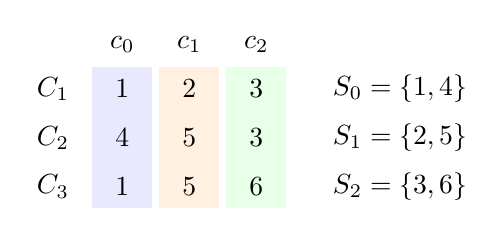
\begin{tikzpicture}[x=.85cm,y=.62cm]
\fill[blue!9](-.45,-2.45) rectangle(.45,.45);
\fill[orange!12](.55,-2.45) rectangle(1.45,.45);
\fill[green!9](1.55,-2.45) rectangle(2.45,.45);
\foreach \x/\lab in {0/0,1/1,2/2}{\node at(\x,.9){$c_{\lab}$};}
\foreach \y/\lab in {0/1,-1/2,-2/3}{\node[anchor=east] at(-.65,\y){$C_{\lab}$};}
\foreach \x/\y/\v in {0/0/1,1/0/2,2/0/3,0/-1/4,1/-1/5,2/-1/3,0/-2/1,1/-2/5,2/-2/6}{\node at(\x,\y){$\v$};}
\node[anchor=west] at(3.0,0){$S_0=\{1,4\}$};
\node[anchor=west] at(3.0,-1){$S_1=\{2,5\}$};
\node[anchor=west] at(3.0,-2){$S_2=\{3,6\}$};
\end{tikzpicture}
\caption{How to read a context--color matrix. Rows are the contexts $123$, $345$, and $561$; column positions are colors. Each occurrence of a repeated vertex stays in its column. Shading denotes the color class, not a new context. Removing repeated entries from a column gives its state support. The $3\times3$ shape does not make this six-vertex array a Latin square. Drawing positions do not specify Hilbert-space ray angles.}\label{fig:matrix-reading}
\end{figure}

In the language of Theorem~\ref{thm:nxd-matrix}, every chromatic phenomenon studied in Ref.~\cite{svozil2026contexts} acquires a transparent matrix interpretation:
\begin{itemize}
\item \emph{Chromatic Gap ($\chi(H)>d$):} No row permutations of $C_1,\ldots,C_n$ can align all shared vertices vertically; every arrangement forces at least one intertwining vertex $v$ to appear in two different columns $j\neq j'$.
\item \emph{Chromatic Inseparability ($u\sim_c v$):} In \emph{every} valid column-aligned $n\times d$ matrix $M$, vertices $u$ and $v$ are forced to occupy the \emph{exact same column}.
\item \emph{Chromatic TIFS ($c(u)\neq c(v)$):} In \emph{every} valid $n\times d$ matrix $M$, $u$ and $v$ are forced into \emph{different columns} (an implicit edge). If some nonextendable state $s\in\Sc(H)\setminus\Sc_{\mathrm{ext}}(H)$ satisfies $s(u)=s(v)=1$, then $\{u,v\}$ can be placed together into a single valid state column $S_0$, but the remaining $n\times(d-1)$ entries cannot be aligned into $d-1$ collision-free columns!
\end{itemize}

\subsection{The Four Barriers to Strict \texorpdfstring{$d\times d$}{d x d} Latin-Square Embedding}\label{sec:barriers}

For this subsection an embedding means an injective map of vertices into the cells of a fixed \emph{net}: rows, columns, and symbol classes of a supplied family of MOLS. Entire contexts must map to entire lines. Different parallel classes of the host meet in exactly one cell. This is stronger than selecting arbitrary transversals or asking whether a partial collection extends to a net. Four necessary obstructions to this specified embedding are as follows; they are not an exhaustive characterization.

\begin{enumerate}
\item \emph{The Linearity Barrier ($|e\cap e'|\ge 2$):} Any two distinct rows, columns, or MOLS transversals in a $d\times d$ grid share at most one cell ($|e\cap e'|\in\{0,1\}$). Thus any non-linear hypergraph ($g(H)=2$), such as $H_{4,2}=\{\{1,2,3\},\{1,2,4\}\}$ or the $4$-dimensional common-apex lifts $W_{11,5}^{(4)},B_{14,7}^{(4)},D_{17,9}^{(4)}$, cannot embed as lines of a $d\times d$ Latin square, while the displayed examples admit an $n\times d$ Context--Color Matrix $M$ (with the shared pair $\{1,2\}$ occupying two fixed columns).
\item \emph{The Grid-Capacity Barrier ($|V|>d^2$ or $|E|>d(d+1)$):} A $d\times d$ grid has only $d^2$ cells and at most $d+1$ parallel classes of $d$ lines (totaling $d(d+1)$ lines when an affine plane of order $d$ exists). Any strongly $d$-colorable hypergraph with $|V|>d^2$—such as an open chain of $n\ge 5$ triads in $d=3$ ($|V|=2n+1\ge 11>9$) or the Yu--Oh restrictions $H_{17,10}$ ($|V|=17>9$) and $H_{21,13}$ ($|V|=21>9$, $|E|=13>12$)—exceeds the capacity of a single $3\times 3$ Latin square, but is represented without loss by a $10\times 3$ or $13\times 3$ Context--Color Matrix.
\item \emph{The Euler--MOLS Barrier ($d=6$):} If $H$ consists of $n=4$ contexts of size $d=6$ that pairwise intersect in a single vertex ($|C_a\cap C_b|=1$ for $1\le a<b\le 4$, with $|V|=\binom{4}{2}+4(6-3)=18\le 36$), then $\chi(H)=6$ because the $6$ shared vertices form the line graph $L(K_4)$, which is $3$-colorable ($\chi'(K_4)=3\le 6$). Thus $H$ has a valid $4\times 6$ Context--Color Matrix, yet cannot embed in a host net of order six: the four pairwise-intersecting contexts require four different complete parallel classes, hence a $6\times 6$ Graeco-Latin square, forbidden by Tarry's theorem.
\item \emph{The Transversal-Closure Barrier (Small Forbidden Configurations):} Even when $H$ is linear ($|e\cap e'|\le 1$), satisfies $|V|\le d^2$ and $|E|\le d(d+1)$, and $d=3$ (where MOLS exist), $H$ can fail to embed into any $3\times 3$ Latin square or $AG(2,3)$ because its contexts violate transversal closure. A $6$-vertex, $4$-context counterexample is the \emph{Pasch configuration} $H_{\mathrm{Pasch}}$, analyzed in detail in Sec.~\ref{sec:pasch}.
\end{enumerate}

% ============================================================================
% ============================================================================
\section{Explicit Constructions from Latin-Square Theorems}\label{sec:constructive}
% ============================================================================

The results in this section supply construction and analysis tools in addition to the matrix representation. We state the imported existence or classification theorem with its source, then prove the hypergraph consequence. A cell is a vertex throughout. In the conventional triple encoding, whose vertices are row labels, column labels, and symbols, transversals are instead perfect matchings and mates are edge colorings; that encoding must not be substituted for the present one. All assertions here are combinatorial unless a ray realization is explicitly supplied.

\subsection{Indivisible plexes: stateless hypergraphs in every uniformity}\label{sec:plexes}

\begin{definition}
In a Latin square of order $n$, a $k$-plex is a set $U$ of $kn$ cells meeting every row, every column, and every symbol class exactly $k$ times. It is \emph{indivisible} if it contains no $t$-plex for any $0<t<k$. Thus a $1$-plex is a transversal. Here $n$ is the square order and $k$, not $n$, will be the hypergraph uniformity.
\end{definition}

\begin{theorem}[Imported indivisible-plex existence theorem]\label{thm:imported-plex}
For every $k\ge2$ and $m\ge1$, there exists a Latin square of order $n=2km$ partitioned into $2m$ disjoint indivisible $k$-plexes~\cite[Theorems 1.1--1.2]{bryant2009indivisible}.
\end{theorem}

\begin{proposition}[Plex-to-hypergraph construction]\label{prop:plex-hypergraph}
Let $U$ be an indivisible $k$-plex in a Latin square $L$ of order $n$, with $k\ge2$. Define
\begin{equation}\label{eq:plex-contexts}
\begin{aligned}
H_U&=(U,E_U),\\
E_U&=\{U\cap R_i,U\cap C_i:i\in[n]\}\\
&\quad\cup\{U\cap S_a^L:0\le a<n\}.
\end{aligned}
\end{equation}
Then $H_U$ is $k$-uniform, linear, and $3$-regular, with $kn$ vertices and $3n$ contexts. It has no two-valued states and $\chi(H_U)>k$. More strongly, no binary assignment sums to $t$ on every context for any $0<t<k$. Consequently, for every uniformity $k\ge2$ there exists such a stateless hypergraph with $2k^2$ vertices and $6k$ contexts.
\end{proposition}
\begin{proof}
Each restricted line has $k$ cells by the plex condition. Distinct original lines meet in at most one cell, and their restrictions cannot coincide because $k\ge2$. Thus all $3n$ contexts are distinct and the hypergraph is linear. Each selected cell belongs to one row, one column, and one symbol context, giving degree three. A binary assignment with exactly $t$ selected cells per context is precisely a $t$-plex contained in $U$, which indivisibility excludes. In particular a state would be a transversal, and a strong $k$-coloring would supply $k$ states. Finally apply Theorem~\ref{thm:imported-plex} with $m=1$.
\end{proof}

This construction preserves linearity while allowing arbitrary uniformity. It does not assert connectedness, criticality, or Hilbert-space realizability. At $k=2$ the resulting objects are stateless graphs; this is not a dimension-two KS claim.

\subsubsection{A complete fifteen-vertex triplex example}

The filled cells in
\begin{equation}\label{eq:triplex-square}
\begin{aligned}
L&=\begin{pmatrix}0&1&2&3&4\\1&0&3&4&2\\2&3&4&0&1\\3&4&1&2&0\\4&2&0&1&3\end{pmatrix},\\
U&=\begin{pmatrix}0&1&2&\cdot&\cdot\\\cdot&0&3&\cdot&2\\\cdot&\cdot&4&0&1\\3&4&\cdot&2&\cdot\\4&\cdot&\cdot&1&3\end{pmatrix}
\end{aligned}
\end{equation}
form a triplex. Number those cells in row order, left to right, from $1$ to $15$. The symbol printed in $U$ is its original Latin symbol, not its vertex number or a proposed hypergraph color. The five row contexts, five column contexts, and five symbol contexts are respectively
\begin{equation}\label{eq:triplex-full-contexts}
\begin{aligned}
E_R={}&\{123,456,789,\{10,11,12\},\{13,14,15\}\},\\
E_C={}&\{\{1,10,13\},\{2,4,11\},\{3,5,7\},\\
&\hspace{8mm}\{8,12,14\},\{6,9,15\}\},\\
E_S={}&\{\{1,4,8\},\{2,9,14\},\{3,6,12\},\\
&\hspace{8mm}\{5,10,15\},\{7,11,13\}\}.
\end{aligned}
\end{equation}
Here $123$ abbreviates $\{1,2,3\}$, and similarly for the other single-digit triples. Direct enumeration of the $5!=120$ row-to-column permutations of $L$ finds no transversal contained in $U$. A $2$-plex inside $U$ would leave a transversal as its complement in $U$, so $U$ is indivisible. Therefore the $15$ contexts above are stateless. The color word in vertex order
\begin{equation}\label{eq:triplex-four-colors}
(0,1,2,2,1,3,0,1,2,2,3,0,1,3,0)
\end{equation}
is injective on every context, proving $\chi(H_U)=4$. This is a fully specified finite example of the plex mechanism, independently verified as described in Appendix~\ref{app:verification}; no novelty or minimum-size claim is intended.

\subsection{Crimped squares: explicit forced color identities}\label{sec:crimped}

The relevant property of a crimped square is a nonvacuous implication between two distinct cells: at least one transversal contains $u$, and every transversal containing $u$ also contains $v$. Danziger, Wanless, and Webb certify such implications by their $\Delta$-crimped constructions and provide examples with orthogonal mates~\cite{danziger2011monogamous}.

\begin{proposition}[Transversal implication gives chromatic identity]\label{prop:crimped-identity}
Suppose $L$ has an orthogonal mate and distinct cells $u,v$ satisfy $s(u)\le s(v)$ for every transversal state of $H_L$. Then $u\sim_c v$. Such colorable examples exist for every odd order $d\ge7$ by the monogamous $\Delta$-crimped constructions of Ref.~\cite[Theorem 3.3]{danziger2011monogamous}.
\end{proposition}
\begin{proof}
For any coloring $c\in\Cc_d(H_L)$, its color class containing $u$ is a transversal. The implication puts $v$ in that same class, so $c(u)=c(v)$. Existence of a mate makes this conclusion nonvacuous. The cited theorem supplies the asserted infinite family.
\end{proof}

This gives an ordinary TITS implication and a chromatic identity. It does not by itself produce a \emph{purely} chromatic gadget: an ordinary implication is already part of the hypothesis, and ordinary state separation must be checked separately.

For a complete published instance, the order-seven square in the proof of that theorem and its displayed mate, with letters renamed $0,\ldots,6$, are
\begin{equation}\label{eq:crimped-seven}
\begin{aligned}
L_{\rm cr}&=\begin{pmatrix}
0&1&2&3&4&5&6\\1&2&0&4&5&6&3\\2&3&4&5&6&0&1\\3&4&1&6&0&2&5\\4&5&6&2&1&3&0\\5&6&3&0&2&1&4\\6&0&5&1&3&4&2
\end{pmatrix},\\
M_{\rm cr}&=\begin{pmatrix}
0&1&2&3&4&5&6\\6&3&4&5&1&2&0\\4&5&6&2&0&1&3\\2&0&5&1&3&6&4\\1&6&3&0&2&4&5\\3&4&1&6&5&0&2\\5&2&0&4&6&3&1
\end{pmatrix}.
\end{aligned}
\end{equation}
Use zero-based coordinates: $u=(5,5)$ and $v=(4,3)$, carrying original symbols $1$ and $2$. The $49$ ordered pairs $(L_{\rm cr},M_{\rm cr})$ are distinct, so $M_{\rm cr}$ is an explicit strong $7$-coloring of the $49$-vertex, $21$-context hypergraph. All $25$ transversals were checked independently: three contain both distinguished cells and none contains exactly one. Thus this particular pair is inseparable already by ordinary states, as well as by colors.

\subsection{Cyclic squares: exact chromatic numbers}\label{sec:cyclic-exact}

\begin{theorem}[Imported cyclic chromatic-number theorem]\label{thm:cyclic-exact}
For $L_d(i,j)=i+j\pmod d$, the $d$-uniform cell hypergraph satisfies
\begin{equation}\label{eq:cyclic-chi}
\chi(H_{L_d})=\begin{cases}d,&d\text{ odd},\\d+2,&d\text{ even}.\end{cases}
\end{equation}
This is the Latin-square graph theorem of Besharati, Goddyn, Mahmoodian, and Mortezaeefar~\cite[Theorem 3]{besharati2016latin}.
\end{theorem}

For odd $d$, $M(i,j)=i+2j\pmod d$ is an explicit mate: multiplication by two is a permutation, and the determinant of the pair of linear forms is one. For even $d$, the summation obstruction in Theorem~\ref{thm:3net} excludes all transversals. Every independent set is then a partial transversal of size at most $d-1$, so
\[
\chi(H_{L_d})\ge\left\lceil\frac{d^2}{d-1}\right\rceil=d+2.
\]
The matching upper bound is the additional imported content of the cited theorem. Thus the result supplies exact chromatic gaps for an infinite family with $d^2$ vertices and $3d$ contexts. It concerns this specific cyclic square, not every square of even order: the Finney example below has chromatic number seven at order six.

\subsection{Finite-field nets: colorings, separation, and saturation}\label{sec:finite-field}

For a prime power $q$, the $q-1$ squares
\begin{equation}\label{eq:field-mols}
L_a(x,y)=x+ay,\qquad a\in\F_q^*,
\end{equation}
are mutually orthogonal. This is the classical complete finite-field MOLS construction~\cite{chowla1960mols}. Choose $A\subseteq\F_q^*$ and form $H_A$ on $\F_q^2$ using the $q$ rows, $q$ columns, and all symbol classes of the squares with $a\in A$. It is a linear $q$-uniform net with $q^2$ vertices and $(|A|+2)q$ contexts.

\begin{proposition}[A controlled finite-field family]\label{prop:field-nets}
Every unused form $L_b$, $b\in\F_q^*\setminus A$, strongly $q$-colors $H_A$. If at least two forms are unused, two such colorings separate all vertices. If exactly one form is unused, $\Gamma(H_A)$ is complete $q$-partite with $q$ parts of size $q$; there is one coloring up to palette permutation, exactly $q$ states, and $q\binom q2$ inseparable pairs. If no form is unused, $\Gamma(H_A)=K_{q^2}$, $\chi(H_A)=q^2$, and $\Sc(H_A)=\varnothing$.
\end{proposition}
\begin{proof}
On a selected line $x+ay=t$, an unused form has value $t+(b-a)y$, a bijection because $b-a\ne0$. It is also bijective on rows and columns because $b\ne0$. Two distinct unused forms have an invertible coefficient matrix, giving distinct joint signatures. With one direction omitted, two cells are nonadjacent exactly when they lie on the same omitted line. Those $q$ lines are the independent parts. A state must be contained in one part and must select $q$ cells to meet every row, hence must be the whole part. With every direction present, every pair is adjacent. A state is then an independent set of size at most one, which cannot meet all $q$ disjoint rows.
\end{proof}

The last additional parallel class changes the strong chromatic number from $q$ to $q^2$. For $q=3$, rows and columns give six contexts; adjoining the $x+y$ symbol classes gives nine contexts with unique coloring $x+2y$ up to palette permutation; adjoining the $x+2y$ classes gives twelve contexts and the graph $K_9$.

These linear nets have no surviving nonextendable states. A state is $T=\{(x,f(x)):x\in\F_q\}$, with $f$ a permutation and each selected $x+af(x)$ also a permutation. For $h\in\F_q$, the translates $T_h=\{(x,f(x)+h)\}$ satisfy the same conditions and partition the cells. Thus every state extends. This is a useful limitation when selecting search families.

For an arbitrary supplied collection of MOLS, a coloring of its row--column--symbol net is exactly a further common orthogonal mate. Hence a maximal collection supplies a chromatic obstruction. Monogamous squares~\cite{danziger2011monogamous} have mates but lie in no triple of MOLS: taking a monogamous pair gives a $d^2$-vertex, $4d$-context net with $\chi>d$. Existence of ordinary states is a separate common-transversal question.

\subsection{Group tables: the Hall--Paige classification}\label{sec:hall-paige}

\begin{theorem}[Imported Hall--Paige classification]\label{thm:hall-paige}
A finite group admits a complete mapping if and only if its Sylow $2$-subgroups are trivial or noncyclic. The necessity is due to Hall and Paige; the sufficiency was completed by Wilcox, Evans, and Bray. We use the statement as summarized in Ref.~\cite[Theorems 1--2]{evans2012strong}.
\end{theorem}

\begin{proposition}[Algebraic state and coloring test]\label{prop:group-test}
For the multiplication table $L_G$ of a group $G$ of order $d$,
\begin{equation}\label{eq:group-classification}
\begin{aligned}
\Sc(H_{L_G})\ne\varnothing
&\iff\chi(H_{L_G})=d\\
&\iff\text{the Sylow $2$-condition holds}.
\end{aligned}
\end{equation}
Whenever states exist, every state extends.
\end{proposition}
\begin{proof}
A transversal is $\{(g,f(g)):g\in G\}$, where both $f(g)$ and $gf(g)$ permute $G$; this is a complete mapping. For every $h\in G$, the cells $\{(g,f(g)h)\}$ again form a transversal, since their symbols are $gf(g)h$. These $d$ translates partition the whole table. Thus every transversal extends to a mate, and Theorem~\ref{thm:hall-paige} gives the classification.
\end{proof}

This avoids a state or coloring enumeration and also rules out group tables as a source of surviving-state gaps or strict state nonextendability. At order four, the cyclic table has no states and chromatic number six; the Klein-four table has states and chromatic number four.

\subsection{Modular defect certificates}\label{sec:delta}

Index the rows, columns, and symbols by $\Z_d$, and put $\Delta(i,j)=L(i,j)-i-j\pmod d$. Summing the three permutations on a transversal gives
\begin{equation}\label{eq:delta-certificate}
\sum_{(i,j)\in T}\Delta(i,j)
\equiv-\frac{d(d-1)}2\pmod d.
\end{equation}
The right side is zero for odd $d$ and $d/2$ for even $d$. The defect method is central to bachelor and crimped constructions~\cite{wanlesswebb2006bachelor,danziger2011monogamous}.

To apply it, list the cells on which $\Delta\ne0$. A transversal must choose a subset of these cells with distinct rows, columns, and symbols, and with the required defect sum. If no such subset exists, there is no state. If no such subset contains $u$, then $s(u)=0$ in every state, excluding an exact-palette coloring. If every such subset containing $u$ also contains $v$, then $s(u)\le s(v)$, and Proposition~\ref{prop:crimped-identity} gives a chromatic identity whenever a mate exists. The compatibility and modular checks are necessary conditions; sufficiency is not assumed. This produces finite arithmetic certificates in place of an unexplained coloring search.

\subsection{Explicit witnesses for the two state/coloring gaps}\label{sec:finite-regimes}

\subsubsection{Finney's order-six square}

The square reproduced by Wanless~\cite{wanless2002plex}, together with an independently checked strong seven-coloring, is
\begin{equation}\label{eq:finney-six}
\begin{aligned}
L_6&=\begin{pmatrix}1&2&3&4&5&6\\2&1&6&5&4&3\\3&4&1&2&6&5\\4&6&5&1&3&2\\5&3&2&6&1&4\\6&5&4&3&2&1\end{pmatrix},\\
C_6&=\begin{pmatrix}0&1&2&3&4&5\\2&3&4&1&0&6\\5&6&1&4&3&0\\4&0&6&5&1&3\\3&4&0&6&2&1\\1&2&5&0&6&4\end{pmatrix}.
\end{aligned}
\end{equation}
All $6!=720$ row-to-column permutations were tested. Exactly $24$ are transversals; every cell occurs in four, and the $36$ cell profiles across these states are distinct. The states are therefore unital and separating. Their disjointness graph has clique counts $24,120,160,30,0$ at sizes one through five. Thus at most four states are pairwise disjoint, excluding a six-coloring by the disjoint-states criterion. Since $C_6$ is proper, $\chi(H_{L_6})=7$.

The fractional chromatic number is six: assign weight $1/4$ to each of the $24$ transversals, covering each cell with total weight one and total cost six; a row clique gives the lower bound. Hence
\[
(\chi,\chi_f,|\Sc|,|\Sc_{\rm ext}|)=(7,6,24,0).
\]
This explicitly realizes a chromatic gap with surviving separating states and no fractional gap.

\subsubsection{An order-seven exact-palette example}

Consider the following square and mate (distinct from the crimped example):
\begin{equation}\label{eq:seven-nonextendable}
\begin{aligned}
L_\star&=\begin{pmatrix}
0&1&2&3&4&5&6\\1&0&3&2&5&6&4\\2&3&0&1&6&4&5\\3&4&5&6&1&2&0\\4&2&6&5&0&3&1\\5&6&1&4&3&0&2\\6&5&4&0&2&1&3
\end{pmatrix},\\
M_\star&=\begin{pmatrix}
0&1&2&3&4&5&6\\2&4&1&5&6&0&3\\3&0&5&4&2&6&1\\6&5&3&1&0&4&2\\1&6&4&0&3&2&5\\4&3&6&2&5&1&0\\5&2&0&6&1&3&4
\end{pmatrix}.
\end{aligned}
\end{equation}
Their orthogonality directly proves $\chi(H_{L_\star})=7$. Exhaustive enumeration gives $63$ states, $49$ extendable states, and eight partitions into seven transversals, hence $8\cdot7!$ labeled colorings. Each cell lies in nine states and all $49$ ordinary-state profiles are distinct.

Using zero-based coordinates, let
\begin{equation}\label{eq:seven-forced-transversal}
T=\{(0,6),(1,4),(2,5),(3,0),(4,1),(5,2),(6,3)\}.
\end{equation}
Among all transversals, the intersection sizes with $T$ are zero, four, and seven, with frequencies $48$, $14$, and one. A partition into transversals must cover exactly seven cells of $T$; without $T$ itself the count would be divisible by four. Thus every coloring contains $T$ as a color class. Precisely the $21=\binom72$ pairs inside $T$ are chromatically inseparable. The fourteen transversals intersecting $T$ in four cells are nonextendable, for instance
\[
\{(0,0),(1,4),(2,5),(3,3),(4,1),(5,2),(6,6)\}.
\]
All $48$ transversals disjoint from $T$ occur in the eight enumerated partitions; together with $T$ they are exactly the $49$ extendable states. The matrices, transversals, and partitions are finite computational examples with the verification procedure specified in Appendix~\ref{app:verification}, not claims of new or minimal Latin squares.

\subsection{Uniformity lifts and the geometric boundary}\label{sec:general-lifts}

\begin{proposition}[Common-apex lift in arbitrary dimension]\label{prop:general-apex}
Let $H$ be $d_0$-uniform and adjoin $r=d-d_0$ common fresh vertices $A$ to every context. Then
\[
\Gamma(H^A)=\Gamma(H)\vee K_r,\qquad\chi(H^A)=\chi(H)+r.
\]
Its states are the old states extended by zero on $A$, together with the $r$ singleton apex states. If $\chi(H)=d_0$, its extendable states transform in the same way, so the old nonextendable states and forced color identities persist. Any injective faithful realization in $\F^{d_0}$ extends faithfully into $\F^d$ by adjoining coordinate rays.
\end{proposition}
\begin{proof}
All new vertices are adjacent to each other and to every old vertex, proving the graph join and chromatic formula. A state either selects one apex, forcing all old vertices to zero, or selects no apex and restricts to an old state. In an exact-palette coloring the apices use $r$ distinct colors absent from the old vertices, leaving precisely $d_0$ colors on $H$. The coordinate construction preserves all old orthogonalities and adds exactly the required ones.
\end{proof}

This propagates the companion's faithful three-dimensional examples to every $d\ge3$, but common apices generally destroy linearity. The plex construction instead preserves linearity but supplies no geometric realization. Uniformity, incidence topology, scalar coloring, and ray geometry are separate requirements. In dimension two every state on a $2$-uniform hypergraph already supplies a binary coloring and extends with its complement, so neither surviving-state chromatic gaps nor nonextendable states occur there.


% ============================================================================
\section{Elementary Building Blocks: Detailed Walkthroughs}\label{sec:elementary}
% ============================================================================

Before turning to the high-complexity quantum configurations of Ref.~\cite{svozil2026contexts}, we present complete, self-contained walkthroughs of the six foundational hypergraph motifs that govern all larger constructions. Table~\ref{tab:elementary-summary} summarizes their invariants.

\begin{table*}[t]
\centering\footnotesize\setlength{\tabcolsep}{3.5pt}
\caption{Summary of elementary building blocks analyzed in Sec.~\ref{sec:elementary}, comparing their $d\times d$ Latin-grid embeddings and $n\times d$ Context--Color Matrix structures.}\label{tab:elementary-summary}
\begin{tabular}{llrrrrrrp{.33\textwidth}}\toprule
Motif & Contexts $E$ & $d$ & $n=|E|$ & $|V|$ & $N_c$ & $|\Sc|$ & $|\Sc_{\mathrm{ext}}|$ & Latin Grid vs.\ $n\times d$ Matrix Structure\\\midrule
$L_{12}$ (Firefly) & $\{123,\,345\}$ & 3 & 2 & 5 & 2 & 5 & 5 & Corner L-hook $R_1\cup C_1$ of $3\times 3$ Latin square; $2\times 3$ matrix; colorings biject with all $12$ order-$3$ Latin squares.\\
$P_3^{(3)}$ (3-Chain) & $\{123,\,345,\,567\}$ & 3 & 3 & 7 & 4 & 8 & 8 & $R_1\cup C_1\cup R_2$ of $3\times 3$ grid; $3\times 3$ matrix with state-size partition $2+2+3=7$.\\
$H_{6,3}$ (Triangle) & $\{123,\,345,\,561\}$ & 3 & 3 & 6 & 1 & 4 & 3 & $R_1\cup C_1\cup S_2^L$ in $3$-net of cyclic $L$; $3\times 3$ matrix; $s_4=\{2,4,6\}$ nonextendable; $1\sim_c 4,2\sim_c 5,3\sim_c 6$.\\
$H_{\mathrm{Pasch}}$ (Pasch) & $\{123,\,145,\,246,\,356\}$ & 3 & 4 & 6 & 1 & 3 & 3 & Unembeddable in any $3\times 3$ Latin square or $AG(2,3)$; clean $4\times 3$ matrix with columns $\{1,6\},\{2,5\},\{3,4\}$.\\
$P_4^{(5)}$ (4-Chain) & $\{1..5,\,5..9,\,9..13,\,13..17\}$ & 5 & 4 & 17 & 13,824 & 185 & 185 & Bipartite path; not an embedding by four complete grid lines; $4\times 5$ matrix (Types I \& II).\\
$C_4^{(5)}$ (4-Cycle) & $\{1..5,\,5..9,\,9..13,\,13..16,1\}$ & 5 & 4 & 16 & 2,808 & 119 & 119 & Exact $R_1,R_2,C_1,C_2$ in $5\times 5$ Latin square with $2\times 2$ hinge block; $4\times 5$ matrix (Types I, II, III).\\
\bottomrule\end{tabular}
\end{table*}

\subsection{The \texorpdfstring{$L_{12}$}{L12} Firefly Lattice: Two Contexts Sharing One Hinge}\label{sec:L12}

The orthomodular lattice $L_{12}$ ($12$ lattice elements: $0,1$, five atoms, and five coatoms, obtained by pasting two Boolean algebras $2^3$ at one common atom and its complement) has the $3$-uniform context hypergraph with $n=2$ contexts and $|V|=5$ vertices:
\begin{equation}\label{eq:L12}
C_1=\{1,2,\mathbf{3}\},\qquad C_2=\{\mathbf{3},4,5\},\qquad C_1\cap C_2=\{\mathbf{3}\}.
\end{equation}

\subsubsection{Embedding as the Corner Hook of a \texorpdfstring{$3\times 3$}{3x3} Latin Square}
Because $C_1$ and $C_2$ intersect at the single hinge vertex $\mathbf{3}$, we assign $C_1$ to Row~1 ($R_1$) and $C_2$ to Column~1 ($C_1$) of a $3\times 3$ Latin square grid, placing the shared hinge $\mathbf{3}$ at the corner cell $(1,1)=R_1\cap C_1$:
\begin{equation}\label{eq:L12-grid}
\begin{array}{c|ccc}
\text{Grid} & \text{Col 1 }(C_2) & \text{Col 2} & \text{Col 3}\\\hline
\text{Row 1 }(C_1) & \mathbf{3}\text{ }(1,1) & 1\text{ }(1,2) & 2\text{ }(1,3)\\
\text{Row 2} & 4\text{ }(2,1) & \cdot\text{ }(2,2) & \cdot\text{ }(2,3)\\
\text{Row 3} & 5\text{ }(3,1) & \cdot\text{ }(3,2) & \cdot\text{ }(3,3)
\end{array}
\end{equation}
Thus $L_{12}$ is literally the ``corner L-hook'' ($R_1\cup C_1$) of a $3\times 3$ Latin square.

\subsubsection{Bijection Between Strong \texorpdfstring{$3$}{3}-Colorings of \texorpdfstring{$L_{12}$}{L12} and \texorpdfstring{$3\times 3$}{3x3} Latin Squares}
To strongly $3$-color $L_{12}$ with palette $\{0,1,2\}$, we choose a color for the hinge $\mathbf{3}$ ($3$ choices), permute the remaining two colors on $\{1,2\}\subset C_1$ ($2!=2$ choices), and independently permute them on $\{4,5\}\subset C_2$ ($2!=2$ choices), yielding $3\times 2\times 2=12$ strong $3$-colorings (or $N_c=2$ normalized colorings fixing $(c(\mathbf{3}),c(1),c(2))=(0,1,2)$).

Remarkably, at $d=3$, \emph{every strong $3$-coloring of $L_{12}$ extends to a unique $3\times 3$ Latin square}: once Row~1 has $(0,1,2)$ and Column~1 has $(0,a,b)$ with $\{a,b\}=\{1,2\}$, cell $(2,3)$ lies in Row~2 (containing $a$) and Column~3 (containing $2$), and cell $(3,2)$ lies in Row~3 (containing $b$) and Column~2 (containing $1$). Row and column uniqueness deterministically force all four remaining cells:
\begin{equation}\label{eq:L12-completions}
L_{\mathrm{A}}=\begin{pmatrix}
\mathbf{0} & \mathbf{1} & \mathbf{2}\\
\mathbf{1} & 2 & 0\\
\mathbf{2} & 0 & 1
\end{pmatrix},\qquad
L_{\mathrm{B}}=\begin{pmatrix}
\mathbf{0} & \mathbf{1} & \mathbf{2}\\
\mathbf{2} & 0 & 1\\
\mathbf{1} & 2 & 0
\end{pmatrix}.
\end{equation}
Hence the $12$ strong $3$-colorings of $L_{12}$ stand in exact one-to-one correspondence with the $12$ Latin squares of order $3$. Moreover, superimposing the two normalized extensions $L_{\mathrm{A}}$ and $L_{\mathrm{B}}$ in Eq.~\eqref{eq:L12-completions} produces a $3\times 3$ Graeco-Latin square $(L_{\mathrm{A}},L_{\mathrm{B}})$ in which all nine color pairs $(a,b)\in\{0,1,2\}^2$ occur once!

\subsubsection{Two-Valued States and the \texorpdfstring{$2\times 3$}{2x3} Context--Color Matrices}
A two-valued state $s\in\Sc(L_{12})$ must satisfy $s(1)+s(2)+s(\mathbf{3})=1$ and $s(\mathbf{3})+s(4)+s(5)=1$:
\begin{itemize}
\item \emph{Case 1 ($s(\mathbf{3})=1$):} Setting the hinge $\mathbf{3}$ to $1$ satisfies both $C_1$ and $C_2$ simultaneously (``$2$-for-$1$''), forcing $s(1)=s(2)=s(4)=s(5)=0$. This gives one state of size $|S_1|=2-(2-1)=1$:
\[
s_1=\{\mathbf{3}\},
\]
which is the restriction to $R_1\cup C_1$ of the two $3\times 3$ permutation matrices passing through $(1,1)$.
\item \emph{Case 2 ($s(\mathbf{3})=0$):} Avoiding the hinge requires choosing one of $\{1,2\}$ in $C_1$ ($2$ choices) and one of $\{4,5\}$ in $C_2$ ($2$ choices), giving $2\times 2=4$ states of size $|S|=2$:
\[
s_2=\{1,4\},\quad s_3=\{2,5\},\quad s_4=\{1,5\},\quad s_5=\{2,4\},
\]
each of which uniquely forces a third cell in $[3]\times[3]\setminus(R_1\cup C_1)$ to form one of the four $3\times 3$ permutation matrices missing $(1,1)$.
\end{itemize}
In Theorem~\ref{thm:nxd-matrix}, the two normalized strong $3$-colorings of $L_{12}$ are represented by the two $2\times 3$ Context--Color Matrices $M_{\mathrm{A}},M_{\mathrm{B}}$ (with $|S_0|+|S_1|+|S_2|=1+2+2=5=|V|$):
\begin{equation}\label{eq:L12-matrices}
M_{\mathrm{A}}=\begin{pmatrix}
\mathbf{c}_0 & \mathbf{c}_1 & \mathbf{c}_2\\\hline
\mathbf{3} & 1 & 2\\
\mathbf{3} & 4 & 5
\end{pmatrix},\qquad
M_{\mathrm{B}}=\begin{pmatrix}
\mathbf{c}_0 & \mathbf{c}_1 & \mathbf{c}_2\\\hline
\mathbf{3} & 1 & 2\\
\mathbf{3} & 5 & 4
\end{pmatrix}.
\end{equation}
Every one of the $5$ states appears as a column in $M_{\mathrm{A}}$ or $M_{\mathrm{B}}$, so $\Sc_{\mathrm{ext}}(L_{12})=\Sc(L_{12})$, and no two vertices are chromatically inseparable because $\{1,4\}$ share column $\mathbf{c}_1$ in $M_{\mathrm{A}}$ but sit in different columns in $M_{\mathrm{B}}$.

\subsection{The Three-Context Open Chain \texorpdfstring{$P_3^{(3)}$}{P3(3)}}\label{sec:P3}

Adjoining a third triad $C_3=\{\mathbf{5},6,7\}$ to $L_{12}$ at vertex $\mathbf{5}$ gives the $3$-context open chain $P_3^{(3)}$ ($d=3,n=3,|V|=7$):
\begin{equation}\label{eq:P3}
C_1=\{1,2,\mathbf{3}\},\qquad C_2=\{\mathbf{3},4,\mathbf{5}\},\qquad C_3=\{\mathbf{5},6,7\}.
\end{equation}
Because $C_1$ and $C_3$ are disjoint while $C_2$ intersects both, the context intersection graph $C_1-C_2-C_3$ is bipartite. In the $3\times 3$ Latin square grid, we assign $C_1=\text{Row 1}$, $C_3=\text{Row 2}$, and $C_2=\text{Column 1}$, placing the two hinges at $\mathbf{3}=(1,1)$ and $\mathbf{5}=(2,1)$:
\begin{equation}\label{eq:P3-grid}
\begin{array}{c|ccc}
\text{Grid} & \text{Col 1 }(C_2) & \text{Col 2} & \text{Col 3}\\\hline
\text{Row 1 }(C_1) & \mathbf{3}\text{ }(1,1) & 1\text{ }(1,2) & 2\text{ }(1,3)\\
\text{Row 2 }(C_3) & \mathbf{5}\text{ }(2,1) & 6\text{ }(2,2) & 7\text{ }(2,3)\\
\text{Row 3} & 4\text{ }(3,1) & \cdot\text{ }(3,2) & \cdot\text{ }(3,3)
\end{array}
\end{equation}

Every two-valued state $s\in\Sc(P_3^{(3)})$ selects exactly one vertex from the middle context $C_2=\{\mathbf{3},4,\mathbf{5}\}$:
\begin{itemize}
\item \emph{Case A ($s(\mathbf{3})=1$):} Satisfies $C_1,C_2$; $C_3$ picks $6$ or $7$, yielding $2$ states of size $2$: $s_1=\{\mathbf{3},6\}$, $s_2=\{\mathbf{3},7\}$.
\item \emph{Case B ($s(\mathbf{5})=1$):} Satisfies $C_2,C_3$; $C_1$ picks $1$ or $2$, yielding $2$ states of size $2$: $s_3=\{1,\mathbf{5}\}$, $s_4=\{2,\mathbf{5}\}$.
\item \emph{Case C ($s(4)=1$, so $s(\mathbf{3})=s(\mathbf{5})=0$):} Satisfies only $C_2$; $C_1$ picks from $\{1,2\}$ and $C_3$ picks from $\{6,7\}$ independently, yielding $2\times 2=4$ states of size $3$: $s_5=\{1,4,6\}$, $s_6=\{1,4,7\}$, $s_7=\{2,4,6\}$, and $s_8=\{2,4,7\}$.
\end{itemize}
In any $3\times 3$ Context--Color Matrix $M$, the three vertices $\{\mathbf{3},\mathbf{5},4\}$ of $C_2$ must occupy distinct columns $\mathbf{c}_0,\mathbf{c}_1,\mathbf{c}_2$. Thus every strong $3$-coloring uses one Case~A state (size $2$), one Case~B state (size $2$), and one Case~C state (size $3$), obeying Eq.~\eqref{eq:size-conservation}: $2+2+3=7=|V|$. Fixing Row~2 ($C_2$) as $(\mathbf{3},\mathbf{5},4)$ yields $2\times 2=4$ normalized $3\times 3$ Context--Color Matrices:
\begin{equation}\label{eq:P3-matrices}
\begin{aligned}
M_1&=\begin{pmatrix}\mathbf{3}&2&1\\\mathbf{3}&\mathbf{5}&4\\6&\mathbf{5}&7\end{pmatrix},&
M_2&=\begin{pmatrix}\mathbf{3}&1&2\\\mathbf{3}&\mathbf{5}&4\\7&\mathbf{5}&6\end{pmatrix},\\[4pt]
M_3&=\begin{pmatrix}\mathbf{3}&1&2\\\mathbf{3}&\mathbf{5}&4\\6&\mathbf{5}&7\end{pmatrix},&
M_4&=\begin{pmatrix}\mathbf{3}&2&1\\\mathbf{3}&\mathbf{5}&4\\7&\mathbf{5}&6\end{pmatrix}.
\end{aligned}
\end{equation}
All $8$ states occur as columns in Eq.~\eqref{eq:P3-matrices}, so $\Sc_{\mathrm{ext}}(P_3^{(3)})=\Sc(P_3^{(3)})$. Notice that $M_1$ and $M_2$ respect the inactive grid columns Col~2 and Col~3 in Eq.~\eqref{eq:P3-grid} ($c(1)\neq c(6)$ and $c(2)\neq c(7)$) and extend directly to full $3\times 3$ Latin squares, whereas $M_3$ and $M_4$ assign the same color to $(1,6)$ or $(2,7)$ because Col~2 and Col~3 are not active contexts in $P_3^{(3)}$ (they become Latin squares upon swapping cells $6\leftrightarrow 7$ in Row~2).

\subsection{The Triangle Hypergraph \texorpdfstring{$H_{6,3}$}{H6,3} and the Cyclic Latin Square \texorpdfstring{$\{\{1,2,3\},\{3,1,2\},\{2,3,1\}\}$}{{{1,2,3},{3,1,2},{2,3,1}}}}\label{sec:triangle}

If we identify vertex $7$ with vertex $1$ in the open chain $P_3^{(3)}$, the chain closes into the $6$-vertex, $3$-context \emph{triangle hypergraph} $H_{6,3}$ (the small-triangle proposition of Ref.~\cite{svozil2026contexts}):
\begin{equation}\label{eq:H63}
C_1=\{\mathbf{1},2,\mathbf{3}\},\qquad C_2=\{\mathbf{3},4,\mathbf{5}\},\qquad C_3=\{\mathbf{5},6,\mathbf{1}\},
\end{equation}
with three degree-$2$ corner hinges $\{\mathbf{1},\mathbf{3},\mathbf{5}\}$ and three degree-$1$ midpoints $\{2,4,6\}$.

\subsubsection{Embedding into the \texorpdfstring{$3$}{3}-Net of the Cyclic Latin Square}
Because $C_1,C_2,C_3$ form an \emph{odd} cycle of contexts ($|C_1\cap C_2|=|C_2\cap C_3|=|C_3\cap C_1|=1$), they cannot be embedded using only rows and columns of a Latin square (whose context intersection graph $K_{d,d}$ is bipartite). By Sec.~\ref{sec:graeco-latin}, $H_{6,3}$ requires \emph{three parallel classes}—one Row, one Column, and one Symbol transversal of a base $3\times 3$ Latin square $L$!

Specifically, take the right-cyclic Latin square $L=\{\{1,2,3\},\{3,1,2\},\{2,3,1\}\}$:
\begin{equation}\label{eq:cyclic-L3}
L=\begin{pmatrix}
1 & \mathbf{2} & 3\\
3 & 1 & \mathbf{2}\\
\mathbf{2} & 3 & 1
\end{pmatrix},
\end{equation}
and select the three contexts from the $3$-net $H_L$:
\begin{itemize}
\item $C_1=\text{Row 1}=\{(1,1),(1,3),(1,2)\}$,
\item $C_2=\text{Column 1}=\{(1,1),(2,1),(3,1)\}$,
\item $C_3=\text{Symbol-}\mathbf{2}\text{ transversal of }L=\{(1,2),(2,3),(3,1)\}$.
\end{itemize}
Their pairwise intersections are the three corners $\mathbf{3}=(1,1)=C_1\cap C_2$, $\mathbf{1}=(1,2)=C_1\cap C_3$, and $\mathbf{5}=(3,1)=C_2\cap C_3$, while the three midpoints are $2=(1,3)\in C_1$, $4=(2,1)\in C_2$, and $6=(2,3)\in C_3$.

\subsubsection{States, the Nonextendable Midpoint State, and the Unique \texorpdfstring{$3\times 3$}{3x3} Matrix}
In $H_{6,3}$, no two corner hinges can both be $1$ because $\{1,3,5\}$ is a $K_3$ clique in $\Gamma(H_{6,3})$:
\begin{itemize}
\item \emph{One corner is $1$ ($3$ states of size $2$):} Setting one corner to $1$ covers two sides of the triangle and forces the opposite midpoint to $1$, yielding
\[
s_1=\{\mathbf{1},4\},\qquad s_2=\{2,\mathbf{5}\},\qquad s_3=\{\mathbf{3},6\}.
\]
\item \emph{All three corners are $0$ ($1$ state of size $3$):} Setting $s(\mathbf{1})=s(\mathbf{3})=s(\mathbf{5})=0$ forces all three midpoints to $1$, yielding
\[
s_4=\{2,4,6\}.
\]
\end{itemize}
Now apply Theorem~\ref{thm:nxd-matrix} to construct a $3\times 3$ Context--Color Matrix $M$ for $H_{6,3}$:
\begin{enumerate}
\item By the size conservation law~\eqref{eq:size-conservation}, the three column state sizes must sum to $|V|=6$. Since the available state sizes are $\{2,2,2,3\}$, the \emph{only} way three state sizes can sum to $6$ is
\[
2+2+2=6,
\]
using $s_1=\{\mathbf{1},4\}$, $s_2=\{2,\mathbf{5}\}$, and $s_3=\{\mathbf{3},6\}$!
\item If we instead try to use $s_4=\{2,4,6\}$ (size $3$) as Column~0 of $M$, the remaining $6-3=3$ vertices $\{\mathbf{1},\mathbf{3},\mathbf{5}\}$ must be placed into the $d-1=2$ remaining columns $\mathbf{c}_1,\mathbf{c}_2$; since $\mathbf{1},\mathbf{3},\mathbf{5}$ pairwise share rows ($C_1,C_2,C_3$), no two can share a column—an immediate Pigeonhole contradiction ($\chi(\Gamma(H_{6,3})[\{1,3,5\}])=3>2$). Thus $s_4\in\Sc(H_{6,3})\setminus\Sc_{\mathrm{ext}}(H_{6,3})$.
\end{enumerate}

Up to column permutation, $H_{6,3}$ therefore admits a \emph{unique} normalized $3\times 3$ Context--Color Matrix $M_{\triangle}$ (and companion cyclically shifted vertex--color square $A_{\triangle}$ via Remark~\ref{rem:vertex-color-array}):
\begin{equation}\label{eq:triangle-matrix}
M_{\triangle}=\begin{pmatrix}
\mathbf{c}_0 & \mathbf{c}_1 & \mathbf{c}_2\\\hline
\mathbf{1} & 2 & \mathbf{3}\\
4 & \mathbf{5} & \mathbf{3}\\
\mathbf{1} & \mathbf{5} & 6
\end{pmatrix},\qquad
A_{\triangle}=\begin{pmatrix}
(\mathbf{1},0) & (2,1) & (\mathbf{3},2)\\
(\mathbf{3},2) & (4,0) & (\mathbf{5},1)\\
(\mathbf{5},1) & (6,2) & (\mathbf{1},0)
\end{pmatrix}.
\end{equation}
In $M_{\triangle}$, the columns lock $\mathbf{1}\sim_c 4$, $2\sim_c\mathbf{5}$, and $\mathbf{3}\sim_c 6$. These colors extend, under the corrected cell dictionary, to the orthogonal mate with rows $(2,0,1)$, $(0,1,2)$, and $(1,2,0)$ of the square in Eq.~\eqref{eq:cyclic-L3}.

\subsection{General \texorpdfstring{$d$}{d}-Uniform Chains \texorpdfstring{$P_m^{(d)}$}{Pm(d)} and the Closed Four-Cycle \texorpdfstring{$C_4^{(5)}$}{C4(5)}}\label{sec:chains-cycles}

Consider now the $5$-uniform $4$-context open chain $P_4^{(5)}$ ($d=5,n=4,|V|=17$):
\begin{equation}\label{eq:P4-5}
\begin{aligned}
C_1&=\{1,2,3,4,\mathbf{5}\},& C_2&=\{\mathbf{5},6,7,8,\mathbf{9}\},\\
C_3&=\{\mathbf{9},10,11,12,\mathbf{13}\},& C_4&=\{\mathbf{13},14,15,16,17\},
\end{aligned}
\end{equation}
and the $16$-vertex closed $4$-cycle $C_4^{(5)}$ obtained by identifying $17\equiv\mathbf{1}$ so that $C_4=\{\mathbf{13},14,15,16,\mathbf{1}\}$ shares hinge $\mathbf{1}$ with $C_1$.

For the closed cycle, assign $C_1=R_1$, $C_3=R_2$, $C_2$ to grid Column~1, and $C_4$ to grid Column~2. Its four hinges occupy the $2\times2$ block $\bigl(\begin{smallmatrix}5&1\\9&13\end{smallmatrix}\bigr)$. This is an injective grid-line embedding. The open chain has \emph{no} such row--column embedding: its context-intersection graph is a four-node path, whereas four selected complete rows and columns would have the additional intersection $C_1\cap C_4$. Splitting that intersection into separate vertices $1$ and $17$ is a useful incidence operation, but no longer an embedding in the original grid. Both hypergraphs are covered by Proposition~\ref{prop:bipartite-completion}.

Using Theorem~\ref{thm:nxd-matrix}:
\begin{itemize}
\item \emph{For the open chain $P_4^{(5)}$ ($|V|=17$):} The $3$ hinges $\{\mathbf{5},\mathbf{9},\mathbf{13}\}$ form a path $5-9-13$. Valid state columns pick an independent set of hinges ($k\in\{0,1,2\}$ active hinges), giving state size $|S|=4-k$:
\begin{enumerate}
\item $k=2$ ($\{\mathbf{5},\mathbf{13}\}$, size $2$): $1$ state;
\item $k=1$ ($\{\mathbf{5}\}$ or $\{\mathbf{13}\}$ with $3\times 4=12$ states each, or $\{\mathbf{9}\}$ with $4\times 4=16$ states; size $3$): $40$ states;
\item $k=0$ ($\varnothing$, size $4$): $4\times 3\times 3\times 4=144$ states;
\end{enumerate}
totaling $|\Sc(P_4^{(5)})|=1+40+144=185$ states. Every $4\times 5$ Context--Color Matrix $M$ distributes the $3$ hinges across the $5$ columns in one of two ways:
\begin{equation}\label{eq:P4-5-matrices}
\begin{aligned}
M_{\mathrm{I}}&=\begin{pmatrix}
\mathbf{5} & 1 & 2 & 3 & 4\\
\mathbf{5} & \mathbf{9} & 6 & 7 & 8\\
\mathbf{13} & \mathbf{9} & 10 & 11 & 12\\
\mathbf{13} & 14 & 15 & 16 & 17
\end{pmatrix}\quad (2+3+4+4+4=17),\\[4pt]
M_{\mathrm{II}}&=\begin{pmatrix}
\mathbf{5} & 1 & 2 & 3 & 4\\
\mathbf{5} & \mathbf{9} & 6 & 7 & 8\\
10 & \mathbf{9} & \mathbf{13} & 11 & 12\\
14 & 15 & \mathbf{13} & 16 & 17
\end{pmatrix}\quad (3+3+3+4+4=17).
\end{aligned}
\end{equation}
All $185$ states extend ($\Sc_{\mathrm{ext}}=\Sc$), with $N_c=(4!)^3=13{,}824$ normalized $4\times 5$ matrices.
\item \emph{For the closed $4$-cycle $C_4^{(5)}$ ($|V|=16$):} The $4$ hinges $\{\mathbf{5},\mathbf{1},\mathbf{9},\mathbf{13}\}$ form a $4$-cycle (the $2\times 2$ Latin corner block), allowing $k=2$ diagonal hinges ($2$ states $\{\mathbf{5},\mathbf{13}\}$ and $\{\mathbf{1},\mathbf{9}\}$ of size $2$), $k=1$ hinge ($4\times 3^2=36$ states of size $3$), or $k=0$ hinges ($3^4=81$ states of size $4$), totaling $|\Sc(C_4^{(5)})|=2+36+81=119$ states. Here the $4\times 5$ Context--Color Matrix has three column-size partitions summing to $16$—Type~I ($2+2+4+4+4=16$, both diagonals monochromatic in the $2\times 2$ block, $1\times(3!)^3=216$ matrices), Type~II ($2+3+3+4+4=16$, one diagonal monochromatic, $6\times(3!)^3=1{,}296$ matrices), and Type~III ($3+3+3+3+4=16$, all four hinges in distinct columns, $6\times(3!)^3=1{,}296$ matrices)—totaling $N_c=13\times 6^3=2{,}808$ normalized matrices, again with $\Sc_{\mathrm{ext}}=\Sc$ by K\H{o}nig's theorem because the $4$-cycle is bipartite!
\end{itemize}

\subsection{The Six-Vertex Pasch Configuration \texorpdfstring{$H_{\mathrm{Pasch}}$}{HPasch}: A \texorpdfstring{$4\times 3$}{4x3} Matrix With No \texorpdfstring{$3\times 3$}{3x3} Latin Square}\label{sec:pasch}

Consider the linear $3$-uniform Pasch hypergraph $H_{\mathrm{Pasch}}$ with $n=4$ contexts and $|V|=6$ degree-$2$ vertices:
\begin{equation}\label{eq:Pasch}
\begin{aligned}
C_1&=\{1,2,3\},\qquad C_2=\{1,4,5\},\\
C_3&=\{2,4,6\},\qquad C_4=\{3,5,6\}.
\end{aligned}
\end{equation}
Every pair of contexts shares a unique vertex. Placing $C_1=\text{Row 1}=\{(1,1),(1,2),(1,3)\}$ and $C_2=\text{Col 1}=\{(1,1),(2,1),(3,1)\}$ in a $3\times 3$ grid fixes $1=(1,1),2=(1,2),3=(1,3),4=(2,1),5=(3,1)$. For $C_3=\{2,4,6\}$ to be a Latin-square transversal through $(1,2)$ and $(2,1)$, its third cell $6$ is forced to be $(3,3)$. Then $C_4=\{3,5,6\}=\{(1,3),(3,1),(3,3)\}$ contains two cells in Row~3 and two cells in Column~3, violating the Latin-square rules! Thus $H_{\mathrm{Pasch}}$ \emph{cannot be embedded into any $3\times 3$ Latin square or $AG(2,3)$}.

Yet in Theorem~\ref{thm:nxd-matrix}, $H_{\mathrm{Pasch}}$ has a unique normalized $4\times 3$ Context--Color Matrix (with $|S_0|+|S_1|+|S_2|=2+2+2=6$ and $\sum_{v\in S_j}\deg(v)=2+2=4=n$):
\begin{equation}\label{eq:Pasch-matrix}
M_{\mathrm{Pasch}}=\begin{pmatrix}
\mathbf{c}_0 & \mathbf{c}_1 & \mathbf{c}_2\\\hline
1 & 2 & 3\\
1 & 5 & 4\\
6 & 2 & 4\\
6 & 5 & 3
\end{pmatrix}\begin{array}{l}
\leftarrow C_1\\
\leftarrow C_2\\
\leftarrow C_3\\
\leftarrow C_4
\end{array},
\end{equation}
whose three columns display the three disjoint states $S_0=\{1,6\}$, $S_1=\{2,5\}$, $S_2=\{3,4\}$ and prove at a glance the forced chromatic identities $1\sim_c 6$, $2\sim_c 5$, and $3\sim_c 4$.

% ============================================================================
\section{Application to Chromatically Complete Configurations and Logical Gadgets (\texorpdfstring{$\chi(H)=d$}{chi(H)=d})}\label{sec:exact-palette}
% ============================================================================

We now apply the $n\times d$ Context--Color Matrix construction systematically to the chromatically complete ($\chi(H)=d$) three- and four-dimensional configurations and logical gadgets of Ref.~\cite{svozil2026contexts} (listed in Tables~I and~II of Ref.~\cite{svozil2026contexts}).

\subsection{The Pentagon \texorpdfstring{$P_5$}{P5} (\texorpdfstring{$5\times 3$}{5x3} Matrix and Purely Chromatic Ternary Exclusion)}\label{sec:P5}

The pentagon hypergraph $P_5$ ($d=3,n=5$ contexts, $|V|=10$, Berge girth $g=5$, real FOR in $\R^3$) has contexts
\begin{equation}\label{eq:P5-contexts}
\begin{aligned}
C_1&=\{1,6,2\},\quad C_2=\{2,7,3\},\quad C_3=\{3,8,4\},\\
C_4&=\{4,9,5\},\quad C_5=\{5,10,1\},
\end{aligned}
\end{equation}
with $5$ degree-$2$ cycle hinges $\{1,2,3,4,5\}$ and $5$ degree-$1$ midpoint vertices $\{6,7,8,9,10\}$.

In a $5\times 3$ Context--Color Matrix $M\in V^{5\times 3}$, each hinge $h\in\{1,2,3,4,5\}$ has $\deg(h)=2$ and saves $1$ vertex when placed in a column [Eq.~\eqref{eq:hinge-saving}]. Because the $5$ hinges form an odd $5$-cycle, at most $\lfloor 5/2\rfloor=2$ nonadjacent hinges can share a single column!
\begin{itemize}
\item \emph{Why $s_{11}=\{6,7,8,9,10\}$ is nonextendable:} The state $s_{11}$ uses $k=0$ hinges (size $|S|=5$). If $s_{11}$ is placed in Column~$\mathbf{c}_0$, the remaining $5$ hinges $\{1,2,3,4,5\}$ must be distributed between only $2$ columns ($\mathbf{c}_1,\mathbf{c}_2$). Since each column can hold at most $2$ hinges, two columns can hold at most $2+2=4<5$ hinges—an immediate Pigeonhole obstruction!
\item \emph{Why all other $10$ states extend ($5$ normalized $5\times3$ matrices):} Every valid $5\times 3$ matrix $M$ must distribute the $5$ hinges across the $3$ columns as $2+2+1=5$ hinges, yielding column support sizes $(5-2)+(5-2)+(5-1)=3+3+4=10=|V|$.
Fixing the anchor context $C_1=(1,6,2)$ in Row~1 as $(\mathbf{c}_0,\mathbf{c}_1,\mathbf{c}_2)=(0,1,2)$ gives the $N_c=5$ normalized $5\times 3$ Context--Color Matrices (corresponding to the $5$ choices of the uniquely colored hinge):
\end{itemize}
\begin{equation}\label{eq:P5-matrices}
\begin{aligned}
M_1^{(P_5)}&=\begin{pmatrix}
\mathbf{1}&6&\mathbf{2}\\
\mathbf{3}&7&\mathbf{2}\\
\mathbf{3}&\mathbf{4}&8\\
9&\mathbf{4}&\mathbf{5}\\
\mathbf{1}&10&\mathbf{5}
\end{pmatrix},&
M_2^{(P_5)}&=\begin{pmatrix}
\mathbf{1}&6&\mathbf{2}\\
\mathbf{3}&7&\mathbf{2}\\
\mathbf{3}&8&\mathbf{4}\\
9&\mathbf{5}&\mathbf{4}\\
\mathbf{1}&\mathbf{5}&10
\end{pmatrix},\\[4pt]
M_3^{(P_5)}&=\begin{pmatrix}
\mathbf{1}&6&\mathbf{2}\\
7&\mathbf{3}&\mathbf{2}\\
\mathbf{4}&\mathbf{3}&8\\
\mathbf{4}&\mathbf{5}&9\\
\mathbf{1}&\mathbf{5}&10
\end{pmatrix},&
M_4^{(P_5)}&=\begin{pmatrix}
\mathbf{1}&6&\mathbf{2}\\
7&\mathbf{3}&\mathbf{2}\\
\mathbf{4}&\mathbf{3}&8\\
\mathbf{4}&9&\mathbf{5}\\
\mathbf{1}&10&\mathbf{5}
\end{pmatrix},\\[4pt]
M_5^{(P_5)}&=\begin{pmatrix}
\mathbf{1}&6&\mathbf{2}\\
7&\mathbf{3}&\mathbf{2}\\
8&\mathbf{3}&\mathbf{4}\\
9&\mathbf{5}&\mathbf{4}\\
\mathbf{1}&\mathbf{5}&10
\end{pmatrix}.
\end{aligned}
\end{equation}
Inspection of Eq.~\eqref{eq:P5-matrices} immediately proves the \emph{purely chromatic ternary exclusion} $\neg(c(6)=c(7)=c(9))$: in any $5\times 3$ matrix where $6,7,9$ all sit in Column~$\mathbf{c}_1$, rows $C_1,C_2,C_4$ force the five hinges $\{1,2,3,4,5\}$ entirely into the two remaining columns $\mathbf{c}_0$ and $\mathbf{c}_2$, which can hold at most $4$ hinges!

\subsection{The Eight-Context Petersen Restriction \texorpdfstring{$H_8$}{H8} (\texorpdfstring{$8\times 3$}{8x3} Matrix)}\label{sec:H8}

Deleting $\{8,2,15\}$ and $\{13,14,15\}$ from Greechie's $G_{32}$~\cite{greechie:71} yields the $14$-vertex, $8$-context hypergraph $H_8$:
\begin{equation}\label{eq:H8-contexts}
\begin{aligned}
C_1&=\{1,2,3\},\ C_2=\{3,4,5\},\ C_3=\{5,6,7\},\\
C_4&=\{7,8,9\},\ C_5=\{9,10,11\},\ C_6=\{11,12,1\},\\
C_7&=\{4,10,13\},\ C_8=\{6,12,14\}.
\end{aligned}
\end{equation}
Here $10$ vertices $\{1,3,4,5,6,7,9,10,11,12\}$ have degree~$2$ and $4$ vertices $\{2,8,13,14\}$ have degree~$1$ ($\sum_{v\in V}\deg(v)=24=8\times 3$).

Anchoring Row~1 ($C_1$) as $(1,2,3)$ across Columns $(\mathbf{c}_0,\mathbf{c}_1,\mathbf{c}_2)$, $H_8$ admits exactly $N_c=3$ normalized $8\times 3$ Context--Color Matrices (corresponding to $c_1,c_2,c_3$ in Supplemental Table~S39 of Ref.~\cite{supplement}):
\begin{equation}\label{eq:H8-matrices}
\begin{aligned}
M_1^{(H_8)}&=\begin{pmatrix}
\mathbf{c}_0&\mathbf{c}_1&\mathbf{c}_2\\\hline
\mathbf{1}&\mathbf{2}&\mathbf{3}\\
\mathbf{4}&5&\mathbf{3}\\
\mathbf{6}&5&\mathbf{7}\\
\mathbf{9}&\mathbf{8}&\mathbf{7}\\
\mathbf{9}&\mathbf{10}&11\\
\mathbf{1}&\mathbf{12}&11\\
\mathbf{4}&\mathbf{10}&\mathbf{13}\\
\mathbf{6}&\mathbf{12}&\mathbf{14}
\end{pmatrix},&
M_2^{(H_8)}&=\begin{pmatrix}
\mathbf{c}_0&\mathbf{c}_1&\mathbf{c}_2\\\hline
\mathbf{1}&\mathbf{2}&\mathbf{3}\\
\mathbf{4}&5&\mathbf{3}\\
\mathbf{6}&5&\mathbf{7}\\
\mathbf{9}&\mathbf{8}&\mathbf{7}\\
\mathbf{9}&11&\mathbf{10}\\
\mathbf{1}&11&\mathbf{12}\\
\mathbf{4}&\mathbf{13}&\mathbf{10}\\
\mathbf{6}&\mathbf{14}&\mathbf{12}
\end{pmatrix},\\[4pt]
M_3^{(H_8)}&=\begin{pmatrix}
\mathbf{c}_0&\mathbf{c}_1&\mathbf{c}_2\\\hline
\mathbf{1}&\mathbf{2}&\mathbf{3}\\
5&\mathbf{4}&\mathbf{3}\\
5&\mathbf{6}&\mathbf{7}\\
\mathbf{9}&\mathbf{8}&\mathbf{7}\\
\mathbf{9}&11&\mathbf{10}\\
\mathbf{1}&11&\mathbf{12}\\
\mathbf{13}&\mathbf{4}&\mathbf{10}\\
\mathbf{14}&\mathbf{6}&\mathbf{12}
\end{pmatrix}.
\end{aligned}
\end{equation}
Looking down the columns of $M_1^{(H_8)},M_2^{(H_8)},M_3^{(H_8)}$ makes the six chromatically inseparable pairs of the Petersen-restriction theorem of Ref.~\cite{svozil2026contexts} visually immediate: in all three matrices,
\begin{itemize}
\item $\{1,9\}$ always co-occur in Column~$\mathbf{c}_0$,
\item $\{2,8\}$ always co-occur in Column~$\mathbf{c}_1$,
\item $\{3,7\}$ always co-occur in Column~$\mathbf{c}_2$,
\item $\{4,6\}$ always share a column ($\mathbf{c}_0$ in $M_1,M_2$; $\mathbf{c}_1$ in $M_3$),
\item $\{10,12\}$ always share a column ($\mathbf{c}_1$ in $M_1$; $\mathbf{c}_2$ in $M_2,M_3$),
\item $\{13,14\}$ always share a column ($\mathbf{c}_2$ in $M_1$; $\mathbf{c}_1$ in $M_2$; $\mathbf{c}_0$ in $M_3$).
\end{itemize}
Across the three matrices, $7$ distinct state supports appear as columns ($\{1,4,6,9\}$ has size $4$; $\{3,7,10,12\}$ has size $4$; $\{2,5,8,10,12\}$, $\{1,5,9,13,14\}$, $\{2,4,6,8,11\}$, $\{3,7,11,13,14\}$ have size $5$; and $\{2,5,8,11,13,14\}$ has size $6$, satisfying $4+5+5=14$ in $M_1,M_3$ and $4+6+4=14$ in $M_2$). The remaining $4$ states of $\Sc(H_8)$ (such as $\{1,5,8,10,14\}$) leave a $5$-cycle in $\Gamma(H_8)[V\setminus S]$ and therefore cannot be completed to an $8\times 3$ matrix.

\subsection{Faithful Yu--Oh Restrictions \texorpdfstring{$H_{17,10}$ and $H_{21,13}$}{H17,10 and H21,13} and the Graeco-Latin Signature Table}\label{sec:H17-H21}

The $17$-ray, $10$-context hypergraph $H_{17,10}$ retains the four base contexts $C_1=\{1,2,3\}$, $C_2=\{7,8,9\}$, $C_3=\{4,5,6\}$, $C_4=\{2,8,5\}$ of completed Yu--Oh $H_{\YO}^+$ together with the six contexts of diagonal sectors $h_1=11$ and $h_2=10$:
\begin{equation}\label{eq:H17-sectors}
\begin{aligned}
\mathcal{E}_{11}&=\bigl\{\{3,11,14\},\{7,11,15\},\{4,11,24\}\bigr\},\\
\mathcal{E}_{10}&=\bigl\{\{9,10,23\},\{1,10,19\},\{4,10,18\}\bigr\}.
\end{aligned}
\end{equation}
Fixing the anchor row $C_4=(2,8,5)$ across columns $(\mathbf{c}_0,\mathbf{c}_1,\mathbf{c}_2)$, $H_{17,10}$ admits $N_c=4$ normalized $10\times 3$ Context--Color Matrices (Table~S41 of Ref.~\cite{supplement}), shown here for $c_1$ and $c_2$:
\begin{equation}\label{eq:H17-matrices}
\setlength{\arraycolsep}{2.2pt}
M_1^{(H_{17,10})}=\begin{pmatrix}
\mathbf{c}_0&\mathbf{c}_1&\mathbf{c}_2\\\hline
2&1&3\\
9&8&7\\
4&6&5\\
2&8&5\\\hline
14&\mathbf{11}&3\\
15&\mathbf{11}&7\\
4&\mathbf{11}&\mathbf{24}\\\hline
9&23&\mathbf{10}\\
19&1&\mathbf{10}\\
4&\mathbf{18}&\mathbf{10}
\end{pmatrix},\ 
M_2^{(H_{17,10})}=\begin{pmatrix}
\mathbf{c}_0&\mathbf{c}_1&\mathbf{c}_2\\\hline
2&1&3\\
9&8&7\\
6&4&5\\
2&8&5\\\hline
\mathbf{11}&14&3\\
\mathbf{11}&15&7\\
\mathbf{11}&4&\mathbf{24}\\\hline
9&23&\mathbf{10}\\
19&1&\mathbf{10}\\
\mathbf{18}&4&\mathbf{10}
\end{pmatrix}.
\end{equation}
In every coloring of $H_{17,10}$, the Specker-bug restriction forces $c(10)\ne c(11)$ (Sec.~\ref{sec:3d-gadgets}). Both hubs are also adjacent to vertex $4$, through the roof contexts $\{4,11,24\}$ and $\{4,10,18\}$. Thus $4,10,11$ always have three distinct colors. The first roof forces $24$ into the color of $10$, and the second forces $18$ into the color of $11$. Hence $10\sim_c24$ and $11\sim_c18$ in all four normalized matrices.

Adjoining the third diagonal sector $\mathcal{E}_{13}=\{\{1,13,20\},\{7,13,21\},\{6,13,22\}\}$ yields $H_{21,13}$ ($n=13$ contexts, $|V|=21$). Only two normalized $13\times 3$ Context--Color Matrices survive ($M_1^{(H_{21,13})}$ and $M_2^{(H_{21,13})}$, corresponding to the antipodal base patterns $101$ and $010$):
\begin{equation}\label{eq:H21-matrices}
\setlength{\arraycolsep}{2.2pt}
M_1^{(H_{21,13})}=\begin{pmatrix}
\mathbf{c}_0&\mathbf{c}_1&\mathbf{c}_2\\\hline
2&1&3\\
9&8&7\\
4&6&5\\
2&8&5\\\hline
14&11&3\\
15&11&7\\
4&11&24\\\hline
9&23&10\\
19&1&10\\
4&18&10\\\hline
13&1&20\\
13&21&7\\
13&6&22
\end{pmatrix},\ 
M_2^{(H_{21,13})}=\begin{pmatrix}
\mathbf{c}_0&\mathbf{c}_1&\mathbf{c}_2\\\hline
2&3&1\\
7&8&9\\
6&4&5\\
2&8&5\\\hline
14&3&11\\
7&15&11\\
24&4&11\\\hline
10&23&9\\
10&19&1\\
10&4&18\\\hline
20&13&1\\
7&13&21\\
6&13&22
\end{pmatrix}.
\end{equation}

The joint-signature criterion of Sec.~\ref{sec:graeco-latin} applies as follows: each vertex $v\in V(H_{21,13})$ receives a $2$-tuple chromatic signature $\sigma(v)=(c_1(v),c_2(v))\in\{0,1,2\}^2$ recording its column index in $M_1^{(H_{21,13})}$ and $M_2^{(H_{21,13})}$. Placing the $21$ vertices into the $3\times 3$ signature grid $\{0,1,2\}\times\{0,1,2\}$ yields the $9$ chromatic equivalence classes:
\begin{equation}\label{eq:H21-signature-grid}
\begin{array}{c|ccc}
c_2\backslash c_1 & \mathbf{c}_0=0 & \mathbf{c}_1=1 & \mathbf{c}_2=2\\\hline
0 & \{2,14\} & \{6\} & \{7,10,20,24\}\\
1 & \{4,13,15,19\} & \{8,23\} & \{3\}\\
2 & \{9\} & \{1,11,18,21\} & \{5,22\}
\end{array}
\end{equation}
Whereas a $3\times 3$ Graeco-Latin square has $9$ vertices and places \emph{one} vertex in each of the $9$ cells of Eq.~\eqref{eq:H21-signature-grid}, $H_{21,13}$ has $21$ vertices and only two normalized colorings, forcing multiple vertices to collide in six of the nine cells and producing the $3\binom{4}{2}+3\binom{2}{2}=21$ chromatically inseparable pairs!

\subsection{Three-Dimensional Logical Gadgets \texorpdfstring{$B_{13,7},D_{16,9},I_{16,9},T_{19,11}$}{B13,7, D16,9, I16,9, T19,11}}\label{sec:3d-gadgets}

The remaining three-dimensional gadgets in the companion inventory~\cite{svozil2026contexts} are sub-hypergraphs or roof extensions of $H_{17,10}$, and their $n\times 3$ Context--Color Matrices directly exhibit how TIFS and TITS constraints operate:

\begin{enumerate}
\item \emph{Completed Specker Bug $B_{13,7}$ ($7\times 3$ matrix, $N_c=6$):} Deleting $C_3=\{4,5,6\}$, $\{4,11,24\}$, and $\{4,10,18\}$ from $H_{17,10}$ leaves the $7$ contexts of $B_{13,7}$:
\[
\begin{aligned}
&\{1,2,3\},\ \{7,8,9\},\ \{2,8,5\},\ \{3,11,14\},\\
&\{7,11,15\},\ \{9,10,23\},\ \{1,10,19\}.
\end{aligned}
\]
Suppose $10$ and $11$ had one common color $h$. Their four neighbors $1,3,7,9$ would all avoid $h$. If $h\ne c(2)$, the context $\{1,2,3\}$ could not contain $h$, contrary to its being rainbow. If $h=c(2)$, then $h\ne c(8)$ because $2,8$ share a context; now $\{7,8,9\}$ cannot contain $h$. Both cases contradict strong coloring. Thus $c(10)\ne c(11)$, without making a palette assumption incompatible with the fixed anchor.
\item \emph{Completed $\Gamma_1$ Gadget $I_{16,9}$ ($9\times 3$ matrix, $N_c=6$):} Re-adjoining the two roof contexts $\{4,11,24\}$ and $\{4,10,18\}$ to $B_{13,7}$ (without $\{4,5,6\}$) appends two rows to each of the $6$ matrices of $B_{13,7}$. Since $10$ and $11$ always occupy distinct columns in $B_{13,7}$, the apex $4$ is forced into the third column, locking $24$ into the column of $10$ ($10\sim_c 24$) and $18$ into the column of $11$ ($11\sim_c 18$).
\item \emph{Purely Chromatic Binary TIFS $D_{16,9}$ ($9\times 3$ matrix, $N_c=7$) and Two-Way TITS $T_{19,11}$ ($11\times 3$ matrix, $N_c=7$):} Deleting $\{1,10,19\}$ from $H_{17,10}$ yields $D_{16,9}$. While the nonextendable state $s=\{1,5,7,14,18,23,24\}\in\Sc(D_{16,9})$ contains both $14$ and $18$, no $9\times 3$ Context--Color Matrix can place $14$ and $18$ in the same column: if $14,18\in\mathbf{c}_0$, then $\{3,11,14\},\{4,11,24\},\{4,10,18\}$ force $3,4$ into one column (say $\mathbf{c}_1$) and $10,11$ into $\mathbf{c}_2$, which forces $7,9\notin\mathbf{c}_2\implies 8\in\mathbf{c}_2$, and $2,5\notin\mathbf{c}_1\implies 2,5\in\mathbf{c}_0$, colliding in Row~4 ($\{2,8,5\}$)! Adjoining the two roof contexts $\{14,26,27\}$ and $\{18,26,28\}$ in $T_{19,11}$ appends two rows to the $7$ normalized $9\times 3$ matrices of $D_{16,9}$; since $14$ and $18$ always sit in distinct columns, their common neighbor $26$ must occupy the third column, locking $28$ into the column of $14$ ($14\sim_c 28$) and $27$ into the column of $18$ ($18\sim_c 27$).
\end{enumerate}

\subsection{Four-Dimensional Apex Lifts and Strictly Linear Gadgets (\texorpdfstring{$n\times 4$}{n x 4} Matrices)}\label{sec:4d-gadgets}

In dimension $d=4$, the $n\times 4$ Context--Color Matrix separates into two distinct structural classes (the companion four-dimensional inventory~\cite{svozil2026contexts}):

\subsubsection{Non-Linear Common-Apex Lifts \texorpdfstring{$W_{11,5}^{(4)}$, $B_{14,7}^{(4)}$, and $D_{17,9}^{(4)}$}{W11,5(4), B14,7(4), and D17,9(4)}}
Each common-apex lift adjoins a single apex vertex $0$ to every $3$-element context $C_i$ of a $3$-dimensional gadget $H$, forming $C_i^{(4)}=\{0\}\cup C_i$. In Theorem~\ref{thm:nxd-matrix}, since $0\in\bigcap_{i=1}^n C_i^{(4)}$ has degree $\deg(0)=n$, Eq.~\eqref{eq:hinge-saving} gives $|S_0|=n-(n-1)=1$. Thus \emph{every} $n\times 4$ Context--Color Matrix $M^{(4)}$ of an apex lift is obtained by prepending a constant Column~$\mathbf{c}_0=(0,0,\ldots,0)^T$ to a valid $n\times 3$ Context--Color Matrix $M^{(3)}$ of $H$:
\begin{equation}\label{eq:apex-matrix}
M^{(4)}=\left(\begin{array}{c|ccc}
\mathbf{c}_0 & \mathbf{c}_1 & \mathbf{c}_2 & \mathbf{c}_3\\\hline
0 & & & \\
0 & & M^{(3)} & \\
\vdots & & & \\
0 & & &
\end{array}\right)\in V^{n\times 4}.
\end{equation}
Equation~\eqref{eq:apex-matrix} provides a one-line matrix proof of the apex-extension proposition of Ref.~\cite{svozil2026contexts}: the normalized coloring count $N_c$ is unchanged, the singleton column $S_0=\{0\}$ is always an extendable state, and the remaining three columns $\mathbf{c}_1,\mathbf{c}_2,\mathbf{c}_3$ are identical to those of $M^{(3)}$.

\subsubsection{Strictly Linear Four-Dimensional Gadgets \texorpdfstring{$W_{16,6}^{(4)}$, $L_{18,7}^{(4)}$, and $L_{22,9}^{(4)}$}{W16,6(4), L18,7(4), and L22,9(4)}}
To restore linearity ($|e\cap e'|\le 1$, so $g(H)\ge 3$), Ref.~\cite{svozil2026contexts} constructs three faithful linear $4$-uniform gadgets in $\R^4$:
\begin{itemize}
\item \emph{Linear $5$-Wheel $W_{16,6}^{(4)}$ ($6\times 4$ matrix, $N_c=80$):} The $6$ contexts are
\[
\begin{aligned}
C_1&=\{2,0,6,1\},\quad C_2=\{2,7,13,3\},\\
C_3&=\{3,0,8,4\},\quad C_4=\{4,9,14,5\},\\
C_5&=\{5,10,15,1\},\quad C_6=\{0,11,12,5\}.
\end{aligned}
\]
Here vertex $0$ lies in only three contexts ($C_1,C_3,C_6$). In any $6\times 4$ matrix $M$, placing $0$ in Column~$\mathbf{c}_3$ covers $0$ in Rows~$1,3,6$. If the three terminals $6,8,11$ were all placed in Column~$\mathbf{c}_0$, then in Rows~$1,3,6$ the outer cycle vertices $\{1,2,3,4,5\}$ would be barred from both $\mathbf{c}_0$ and $\mathbf{c}_3$! Thus $\{1,2,3,4,5\}$ would have to be distributed across only two columns ($\mathbf{c}_1,\mathbf{c}_2$) while pairwise sharing rows around the $5$-cycle $C_1-C_2-C_3-C_4-C_5$, which is impossible. One explicit $6\times4$ matrix is:
\begin{equation}\label{eq:W16-matrix}
M_1^{(W_{16,6}^{(4)})}=\begin{pmatrix}
\mathbf{c}_0 & \mathbf{c}_1 & \mathbf{c}_2 & \mathbf{c}_3\\\hline
2 & \mathbf{0} & \mathbf{6} & 1\\
2 & 7 & 3 & 13\\
\mathbf{8} & \mathbf{0} & 3 & 4\\
5 & 9 & 14 & 4\\
5 & 10 & 15 & 1\\
5 & \mathbf{0} & \mathbf{11} & 12
\end{pmatrix}.
\end{equation}
\item \emph{Linear Quaternion TIFS $L_{18,7}^{(4)}$ ($7\times 4$ matrix, $N_c=144$, $\Sc_{\mathrm{ext}}=\Sc=68$) and Linear TITS $L_{22,9}^{(4)}$ ($9\times 4$ matrix, $N_c=216$):} In $L_{18,7}^{(4)}$, the $7$ contexts are
\[
\begin{aligned}
C_1&=\{1,2,4,3\},\ C_2=\{5,8,7,6\},\ C_3=\{4,9,10,8\},\\
C_4&=\{11,1,12,5\},\ C_5=\{11,14,13,2\},\\
C_6&=\{15,3,16,7\},\ C_7=\{15,17,18,6\}.
\end{aligned}
\]
Why can $11$ and $15$ never share a column in a $7\times 4$ matrix (or even a single state column)? If $11,15\in\mathbf{c}_0$, then Rows~$4,5,6,7$ bar $\{1,2,3\}$ and $\{5,6,7\}$ from $\mathbf{c}_0$; then Row~1 ($\{1,2,4,3\}$) forces $4\in\mathbf{c}_0$ and Row~2 ($\{5,8,7,6\}$) forces $8\in\mathbf{c}_0$, so $4$ and $8$ collide in Column~$\mathbf{c}_0$ of Row~3 ($\{4,9,10,8\}$)! In $L_{22,9}^{(4)}$, adjoining $C_8=\{11,21,22,19\}$ and $C_9=\{13,20,15,19\}$ whose listed context $C_9$ includes the pair $\{13,15\}$ ensures that $\{11,13,15,19\}$ occupy all four distinct columns, locking $20\in C_9$ into the column of $11$ ($11\sim_c 20$). An explicit $9\times 4$ Context--Color Matrix (with its first context fixed as $(1,2,3,4)$) is:
\begin{equation}\label{eq:L22-matrix}
M_1^{(L_{22,9}^{(4)})}=\begin{pmatrix}
\mathbf{c}_0 & \mathbf{c}_1 & \mathbf{c}_2 & \mathbf{c}_3\\\hline
1 & 2 & 3 & 4\\
7 & 5 & 8 & 6\\
9 & 10 & 8 & 4\\
1 & 5 & \mathbf{11} & 12\\
13 & 2 & \mathbf{11} & 14\\
7 & 15 & 3 & 16\\
17 & 15 & 18 & 6\\
21 & 22 & \mathbf{11} & 19\\
13 & 15 & \mathbf{20} & 19
\end{pmatrix}.
\end{equation}
Notice how Column~$\mathbf{c}_2$ in Eq.~\eqref{eq:L22-matrix} locks $\mathbf{11}$ (in Rows~$4,5,8$) and $\mathbf{20}$ (in Row~$9$) into the same state column $S_2=\{3,8,11,18,20\}$.
\end{itemize}

% ============================================================================
\section{Application to Chromatically Incomplete Configurations (\texorpdfstring{$\chi(H)>d$}{chi(H)>d}): Column Collisions and Latin Skeletons}\label{sec:obstructions}
% ============================================================================

We now turn to Regime~I of Ref.~\cite{svozil2026contexts}—the chromatically incomplete hypergraphs ($\chi(H)>d$, $\Cc_d(H)=\varnothing$)—and show how the $n\times d$ Context--Color Matrix and Latin-square theory explain their obstructions.

\subsection{\texorpdfstring{$H_9$}{H9} and Greechie's Petersen Hypergraph \texorpdfstring{$G_{32}$}{G32} (\texorpdfstring{$9\times 3$ and $10\times 3$}{9x3 and 10x3} Column Collisions)}\label{sec:G32}

Recall from Sec.~\ref{sec:H8} that in \emph{every} valid $8\times 3$ Context--Color Matrix of $H_8$ [Eq.~\eqref{eq:H8-matrices}], vertices $2$ and $8$ are locked into the \emph{exact same column} ($2\sim_c 8$), and vertices $13$ and $14$ are locked into the \emph{exact same column} ($13\sim_c 14$).
\begin{itemize}
\item \emph{Why $\chi(H_9)=4$:} $H_9$ adjoins a $9$th row $C_9=\{8,2,15\}$ to $H_8$. By Row Bijectivity, $2$ and $8$ must be placed in \emph{different} columns of Row~9, whereas Rows~1--8 force $2$ and $8$ into the \emph{same} column—an immediate column collision!
\item \emph{Why $\chi(G_{32})=4$ from state intersection:} $G_{32}$ further adjoins Row~10, $C_{10}=\{13,14,15\}$ (producing a second collision $13\sim_c 14$). From the column-state perspective of Theorem~\ref{thm:nxd-matrix}, each vertex in $G_{32}$ has $\deg(v)=2$, so by Eq.~\eqref{eq:deg-conservation} any state column $S_j$ in a $10\times 3$ matrix must have size $|S_j|=10/2=5$. However, the $|\Sc(G_{32})|=6$ state supports of size $5$ pairwise intersect in one vertex ($|S_\alpha\cap S_\beta|=1$ for $\alpha\neq\beta$)~\cite{svozil2026contexts}, so not even \emph{two} disjoint columns exist! A strong 4-coloring can instead be recorded in a $10\times4$ matrix with one blank per row (Remark~\ref{rem:wider-palette}). Its columns are independent sets, not four disjoint states. The lower-bound argument proves $\chi\ge4$; the companion supplies a 4-coloring and hence equality.
\end{itemize}

\subsection{Completed Yu--Oh \texorpdfstring{$H_{\YO}^+$}{HYO+} (\texorpdfstring{$16\times 3$}{16x3} Obstruction) and \texorpdfstring{$H_{\YO}^{(4)}$}{HYO(4)}}\label{sec:HYO}

Completed Yu--Oh $H_{\YO}^+$ has $n=16$ contexts of size $d=3$ on $|V|=25$ vertices: the $4\times 3$ base block $E_{\mathrm{base}}=\{\{1,2,3\},\{7,8,9\},\{4,5,6\},\{2,8,5\}\}$ and four $3\times 3$ diagonal sector blocks $\mathcal{E}_{h}$ ($h\in\{10,11,12,13\}$), where each $\mathcal{E}_h$ consists of three rows $\{x,h,w_{xh}\}$ for $x\in N(h)$.

In a $16\times 3$ Context--Color Matrix $M$:
\begin{enumerate}
\item In each $3\times 3$ sector block $\mathcal{E}_h$, the hub $h$ appears in all three rows and must therefore occupy a \emph{single column} $j_h\in\{\mathbf{c}_0,\mathbf{c}_1,\mathbf{c}_2\}$.
\item By Row Bijectivity, none of the three neighbors $x\in N(h)$ can occupy column $j_h$! That is, the three neighbors $N(h)\subset\{1,3,4,6,7,9\}$ are restricted to the \emph{two remaining columns} $\{0,1,2\}\setminus\{j_h\}$.
\item However, in the $4\times 3$ base block (fixing Row~4 as $(2,8,5)$), there are only $2^3=8$ ways to order the pairs $\{1,3\},\{7,9\},\{4,6\}$ across the two available columns in Rows~1, 2, and 3:
\begin{equation}\label{eq:YO-base-matrix}
M_{\mathrm{base}}(b_1,b_2,b_3)=\begin{pmatrix}
\mathbf{c}_0 & \mathbf{c}_1 & \mathbf{c}_2\\\hline
2 & 1\text{ or }3 & 3\text{ or }1\\
9\text{ or }7 & 8 & 7\text{ or }9\\
6\text{ or }4 & 4\text{ or }6 & 5\\
2 & 8 & 5
\end{pmatrix}.
\end{equation}
As shown in the base-coloring partition theorem of Ref.~\cite{svozil2026contexts}, each of the $8$ choices of $(b_1,b_2,b_3)\in\{0,1\}^3$ places one of the four triples $N(10)=\{1,9,4\}$, $N(11)=\{3,7,4\}$, $N(12)=\{3,9,6\}$, or $N(13)=\{1,7,6\}$ across \emph{all three columns} $\mathbf{c}_0,\mathbf{c}_1,\mathbf{c}_2$—leaving \emph{zero} available columns for the corresponding hub $h_j$!
\end{enumerate}
Consequently, no $16\times 3$ Context--Color Matrix exists ($\chi(H_{\YO}^+)=4$). Appending the common apex $26$ in $H_{\YO}^{(4)}$ prepends the singleton column $\mathbf{c}_0=(26,\ldots,26)^T$ as in Eq.~\eqref{eq:apex-matrix}, shifting the exact same obstruction to $16\times 4$ ($\chi(H_{\YO}^{(4)})=5$).

\subsection{The \texorpdfstring{$37$}{37}-Ray Complex Hesse Hypergraph \texorpdfstring{$H_{37}$}{H37}: An Affine-Plane / MOLS Obstruction}\label{sec:H37}

The $37$-ray, $24$-context complex Hesse hypergraph $H_{37}$ in $\C^3$ (the Hesse section of Ref.~\cite{svozil2026contexts}) provides a context hypergraph organized by a finite-geometry Latin-square / MOLS skeleton.

Consider the $9$ core vertices $M_{ak}$ ($a,k\in\Z_3$), arranged as a $3\times 3$ grid:
\begin{equation}\label{eq:H37-grid}
\begin{array}{c|ccc}
M_{ak} & k=0 & k=1 & k=2\\\hline
a=0\ (\mathcal{M}_0) & M_{00}\ (2) & M_{01}\ (3) & M_{02}\ (4)\\
a=1\ (\mathcal{M}_1) & M_{10}\ (5) & M_{11}\ (6) & M_{12}\ (7)\\
a=2\ (\mathcal{M}_2) & M_{20}\ (8) & M_{21}\ (9) & M_{22}\ (10)
\end{array}
\end{equation}
The grid columns $N(P_k)$ and cyclic symbol classes $N(Q_k)$ below are neighborhoods, not contexts. They must omit a color, whereas the actual row contexts must be rainbow. Thus these patterns do not make the core into a $3$-net hypergraph $H_L$.

Look at how the $24$ contexts of $H_{37}$ [the listed Hesse contexts in Ref.~\cite{svozil2026contexts}] act on this $3\times 3$ grid in a putative $24\times 3$ Context--Color Matrix:
\begin{enumerate}
\item \emph{Rows of the $3\times 3$ Grid ($\mathcal{M}_a=\{M_{a0},M_{a1},M_{a2}\}$):} The first $3$ contexts $\mathcal{M}_0,\mathcal{M}_1,\mathcal{M}_2$ are the \emph{rows} of Eq.~\eqref{eq:H37-grid}, forcing each row of Eq.~\eqref{eq:H37-grid} to contain all three colors $\{\mathbf{c}_0,\mathbf{c}_1,\mathbf{c}_2\}$.
\item \emph{Columns of the $3\times 3$ Grid ($\mathcal{B}_{ak}=\{M_{ak},P_k,B_{ak}\}$):} For each fixed $k\in\Z_3$, vertex $P_k$ appears in $\mathcal{B}_{0k},\mathcal{B}_{1k},\mathcal{B}_{2k}$ alongside the $k$th \emph{column} $N(P_k)=\{M_{0k},M_{1k},M_{2k}\}$ of Eq.~\eqref{eq:H37-grid}. Thus column $k$ of the grid~\eqref{eq:H37-grid} must omit the color $c(P_k)$!
\item \emph{Cyclic Latin-Square Transversals ($\mathcal{C}_{ak}=\{M_{a,a+k},Q_k,C_{ak}\}$):} For each fixed $k\in\Z_3$, vertex $Q_k$ appears alongside the diagonal transversal
\[
N(Q_k)=\{M_{0,k},\,M_{1,k+1},\,M_{2,k+2}\},
\]
which is the $k$th symbol class of the cyclic Latin square $L(a,\ell)=\ell-a\pmod 3$! Thus each cyclic diagonal $N(Q_k)$ must omit the color $c(Q_k)$.
\item \emph{The Apex Constraint ($\mathcal{A}_k=\{z,P_k,A_k\}$):} Fix $z$ in Column~$\mathbf{c}_0$ ($c(z)=0$). Then the three rows $\mathcal{A}_0,\mathcal{A}_1,\mathcal{A}_2$ bar $P_0,P_1,P_2$ from Column~$\mathbf{c}_0$, so $c(P_k)\in\{1,2\}$.
\end{enumerate}

Now watch how the Latin-square structure produces the contradiction $\chi(H_{37})=4$:
\begin{itemize}
\item If $P_0,P_1,P_2$ all had the same color (say $1$), then by (2) no entry $M_{ak}$ in any column of Eq.~\eqref{eq:H37-grid} could have color $1$, contradicting (1) that every row $\mathcal{M}_a$ contains all three colors!
\item Hence $\{c(P_0),c(P_1),c(P_2)\}=\{1,2\}$. Up to a cyclic shift of the column index $k\in\Z_3$ and exchanging colors $1,2$, set $(c(P_0),c(P_1),c(P_2))=(2,1,1)$.
\item Since Column~$0$ of Eq.~\eqref{eq:H37-grid} omits color $2$, and Columns~$1$ and~$2$ omit color $1$, the unique color-$1$ entry in each row $\mathcal{M}_a$ \emph{must sit in Column~$0$} ($c(M_{a0})=1$ for all $a\in\Z_3$), while the remaining two entries $(M_{a1},M_{a2})$ in each row must be a permutation $(x_a,2-x_a)$ of $\{0,2\}$:
\begin{equation}\label{eq:H37-forced-grid}
c(M)=\begin{pmatrix}
1 & x_0 & 2-x_0\\
1 & x_1 & 2-x_1\\
1 & x_2 & 2-x_2
\end{pmatrix},\qquad x_a\in\{0,2\}.
\end{equation}
\item Now read off the three cyclic Latin-square transversals $N(Q_k)$ from Eq.~\eqref{eq:H37-forced-grid}:
\[
\begin{aligned}
c(N(Q_0))&=\{1,\,x_1,\,2-x_2\},\\
c(N(Q_1))&=\{x_0,\,2-x_1,\,1\},\\
c(N(Q_2))&=\{2-x_0,\,1,\,x_2\}.
\end{aligned}
\]
By (3), none of these three transversals can be rainbow ($\{0,1,2\}$), so the two non-$1$ entries in each transversal must be equal:
\[
x_1=2-x_2,\qquad x_0=2-x_1,\qquad x_2=2-x_0,
\]
which requires $x_0=2-x_1=2-(2-x_2)=x_2=2-x_0\implies x_0=1\notin\{0,2\}$, a contradiction!
\end{itemize}
Thus no $24\times3$ Context--Color Matrix exists, proving $\chi(H_{37})\ge4$. A strong four-coloring is explicit: set $c(P_k)=c(Q_k)=3$, $c(z)=0$, $c(A_k)=1$, $c(M_{ak})=k$, $c(B_{ak})=k+1\pmod3$, and $c(C_{ak})=a+k+1\pmod3$. Every listed context has three distinct colors. This supplies the upper bound and proves $\chi(H_{37})=4$; its four-column matrix has one blank per row.

\subsection{The Four-Dimensional Completion \texorpdfstring{$H_{65}$}{H65} (\texorpdfstring{$29\times 4$}{29x4} Pigeonhole Overflow)}\label{sec:H65}

Finally, consider the canonical linear $4$-uniform hypergraph $H_{65}$ in $\R^4$ ($|V|=65,n=29$ contexts, the real-completion section of Ref.~\cite{svozil2026contexts}), built from the $17$-ray core $V_{\mathrm{core}}=\{1,\ldots,17\}$ with $5$ core contexts
\begin{equation}\label{eq:H65-core}
\begin{aligned}
C_1&=\{1,2,3,4\},\ C_2=\{5,6,7,8\},\ C_3=\{9,10,12,13\},\\
C_4&=\{9,11,14,15\},\ C_5=\{10,11,16,17\},
\end{aligned}
\end{equation}
and $24$ completed bridge contexts $E_m=\{u_m,v_m,2m+16,2m+17\}$ ($1\le m\le 24$).

In the $29\times 4$ Context--Color Matrix picture of Theorem~\ref{thm:nxd-matrix}, the non-4-colorability $\chi(H_{65})=5$ (despite $H_{65}$ having $|\Sc(H_{65})|=393{,}216$ two-valued states!) has a one-line Pigeonhole proof:
\begin{enumerate}
\item Every state column $S_j$ in a $29\times 4$ Context--Color Matrix must be an independent set of $\Gamma(H_{65})$.
\item On the $17$-vertex core $V_{\mathrm{core}}$, the independence number is $\alpha(G_{\mathrm{core}})=4$: every state $s\in\Sc(H_{65})$ selects \emph{at most $4$ core vertices} (in fact $|S_j\cap V_{\mathrm{core}}|=4$: one from $C_1$, one from $C_2$, one hub from $\{9,10,11\}$, and one bridge ray from $B_1\cup B_2\cup B_3$).
\item Therefore, four disjoint state columns $S_0,S_1,S_2,S_3$ can cover at most
\begin{equation}\label{eq:H65-pigeonhole}
\sum_{j=0}^{3}\bigl|S_j\cap V_{\mathrm{core}}\bigr|\le 4\times 4=16 < 17=\bigl|V_{\mathrm{core}}\bigr|
\end{equation}
core vertices. At least one of the $17$ core vertices is left without a column, proving $\chi(H_{65})\ge5$. The companion supplies a five-coloring, giving $\chi(H_{65})=5$. Such a five-column representation has one blank per row; its columns are independent sets, as in Remark~\ref{rem:wider-palette}.
\end{enumerate}

Similarly, in the transverse chromatic-to-stateless extension $T(H)$ (the transverse-extension proposition of Ref.~\cite{svozil2026contexts}), taking $d-1$ disjoint copies $H^{(1)},\ldots,H^{(d-1)}$ linked by transverse contexts $T_v=\{v^{(1)},\ldots,v^{(d-1)},w_v\}$ directly materializes the first $d-1$ columns $\mathbf{c}_0,\ldots,\mathbf{c}_{d-2}$ of the $n\times d$ Context--Color Matrix as the state supports on $H^{(1)},\ldots,H^{(d-1)}$, while the fresh vertices $w_v$ encode the $d$th column $\mathbf{c}_{d-1}$ via $s(w_v)=1-\sum_{k=1}^{d-1}s(v^{(k)})$.

% ============================================================================
\begin{remark}[Two arrays with different index sets]\label{rem:two-arrays}
The context--color matrix has $n=|E|$ rows and $d$ columns; its entries are original vertices, with repetitions at shared contexts. The transverse-copy array has $d$ rows and $|V|$ columns: rows $1,\ldots,d-1$ contain the copied vertices $v^{(a)}$, and row $d$ contains $w_v$. They are related by a state/coloring bijection. A state on the transverse construction selects one entry in every original-vertex column; its row index defines $c(v)$, using the relabeled palette $[d]$. For every original context $e$ and $a<d$, the state equation on $e^{(a)}$ selects exactly one vertex with $c(v)=a$. The remaining vertex has color $d$, since
\[
\sum_{v\in e}s(w_v)=d-\sum_{a=1}^{d-1}\sum_{v\in e}s(v^{(a)})=1.
\]
Conversely, a strong coloring selects these copied entries and satisfies every state equation. No geometric realization of the transverse construction is implied by this combinatorial correspondence.
\end{remark}

\section{Summary and Conclusion}\label{sec:conclusion}
% ============================================================================

Table~\ref{tab:master-matrix-synthesis} synthesizes the Latin-square and $n\times d$ Context--Color Matrix properties across all configurations analyzed in this paper and in Ref.~\cite{svozil2026contexts}.

\begin{table*}[t]
\centering\footnotesize\setlength{\tabcolsep}{2.5pt}
\caption{Synthesis of the $n\times d$ Context--Color Matrix and Latin-square / MOLS structures across the elementary motifs and the principal three- and four-dimensional configurations of Ref.~\cite{svozil2026contexts}. Here $L_d$ is the number of labeled Latin squares and $m_L$ the number of labeled mates of $L$; $N_c$ is normalized by palette permutations.}\label{tab:master-matrix-synthesis}
\begin{tabular}{llrrrrp{.39\textwidth}}\toprule
Configuration & $d$ & $n\times d$ & $|V|$ & $N_c$ & $|\Sc_{\mathrm{ext}}|/|\Sc|$ & Matrix Mechanism and Latin / MOLS Interpretation\\\midrule
$H_{d\times d}$ (Grid) & $d$ & $2d\times d$ & $d^2$ & $L_d/d!$ & $d!/d!$ & Folds into $d\times d$ Latin square; columns are permutation matrices; K\H{o}nig's theorem ensures $\Sc_{\mathrm{ext}}=\Sc$.\\
$H_L$ ($3$-Net) & $d$ & $3d\times d$ & $d^2$ & $m_L/d!$ & Transv. & States are transversals of $L$; colorings are orthogonal mates (Graeco-Latin squares); realizes all $3$ contextual regimes.\\
$L_{12}$ (Firefly) & 3 & $2\times 3$ & 5 & 2 & $5/5$ & Corner L-hook $R_1\cup C_1$; column sizes $1+2+2=5$; colorings biject with the $12$ Latin squares of order $3$.\\
$P_3^{(3)}$ (3-Chain) & 3 & $3\times 3$ & 7 & 4 & $8/8$ & $R_1\cup C_1\cup R_2$; column sizes $2+2+3=7$; $2$ matrices are partial Latin squares, $2$ swap free column cells.\\
$H_{6,3}$ (Triangle) & 3 & $3\times 3$ & 6 & 1 & $3/4$ & $R_1\cup C_1\cup S_2^L$ in cyclic $3$-net; $2+2+2=6$; midpoint state $\{2,4,6\}$ leaves $K_3$; locks $1\sim_c 4,2\sim_c 5,3\sim_c 6$.\\
$H_{\mathrm{Pasch}}$ (Pasch) & 3 & $4\times 3$ & 6 & 1 & $3/3$ & Fails transversal closure in any $3\times 3$ Latin square; unique $4\times 3$ matrix with columns $\{1,6\},\{2,5\},\{3,4\}$.\\
$P_4^{(5)}$ / $C_4^{(5)}$ & 5 & $4\times 5$ & $17/16$ & $13{,}824/2{,}808$ & $185,\,119$ & Bipartite path / grid-embedded cycle; context-intersection theorem ensures $\Sc_{\mathrm{ext}}=\Sc$.\\
$P_5$ (Pentagon) & 3 & $5\times 3$ & 10 & 5 & $10/11$ & Column sizes $3+3+4=10$; midpoint state $\{6..10\}$ leaves $C_5$; ternary exclusion $\neg(c(6)=c(7)=c(9))$.\\
$H_8$ (Petersen$-2$) & 3 & $8\times 3$ & 14 & 3 & $7/11$ & Column sizes $4+5+5$ or $4+6+4$; locks $6$ pairs including $2\sim_c 8$ and $13\sim_c 14$ across all $3$ matrices.\\
$H_9$ / $G_{32}$ & 3 & $9/10\times 3$ & 15 & 0 & $0/8,\,0/6$ & Row $\{8,2,15\}$ collides with column-locked $2\sim_c 8$ of $H_8$; $G_{32}$ states of size $5$ pairwise intersect ($\chi=4$).\\
$B_{13,7}$ / $I_{16,9}$ & 3 & $7/9\times 3$ & $13/16$ & 6 & $12/14,\,12/22$ & $10$ and $11$ never share a column in $B_{13,7}$, forcing $4$ into third column and locking $10\sim_c 24,11\sim_c 18$ in $I_{16,9}$.\\
$D_{16,9}$ / $T_{19,11}$ & 3 & $9/11\times 3$ & $16/19$ & 7 & $14/21,\,14/25$ & Purely chromatic $c(14)\neq c(18)$ in $D_{16,9}$ forces roof apex $26$ into third column, locking $14\sim_c 28,18\sim_c 27$.\\
$H_{17,10}$ & 3 & $10\times 3$ & 17 & 4 & $10/18$ & Locks $10\sim_c 24,11\sim_c 18$; Born vector $p_{24}=1\neq 8/9=p_{10}$ forces $\eta=1/9$ non-column state weight.\\
$H_{21,13}$ & 3 & $13\times 3$ & 21 & 2 & $6/21$ & Pair of $13\times 3$ matrices induces $3\times 3$ Graeco-Latin signature grid with $21$ colliding pairs ($15$ two-way).\\
$H_{\YO}^+$ / $H_{\YO}^{(4)}$ & $3/4$ & $16\times 3/4$ & $25/26$ & 0 & $0/24,\,0/25$ & Each of $8$ base-block alignments makes one $N(h_j)$ span all $3$ columns, blocking $h_j$ ($\chi=d+1$).\\
$W_{11,5}^{(4)},B_{14,7}^{(4)},D_{17,9}^{(4)}$ & 4 & $n\times 4$ & $11/14/17$ & $5/6/7$ & $11/12,13/15,15/22$ & Common-apex lifts prepend constant singleton column $\mathbf{c}_0=(0,\ldots,0)^T$ to $M^{(3)}$.\\
$W_{16,6}^{(4)},L_{18,7}^{(4)},L_{22,9}^{(4)}$ & 4 & $6/7/9\times 4$ & $16/18/22$ & $80/144/216$ & $56/72,68/68,92/158$ & Linear $4$D gadgets; $L_{18,7}^{(4)}$ has $\Sc_{\mathrm{ext}}=\Sc$; $L_{22,9}^{(4)}$ locks $11\sim_c 20$ in one column.\\
$H_{37}$ (Hesse) & 3 & $24\times 3$ & 37 & 0 & $0/153$ & Core $M_{ak}$ has a $3$-net incidence skeleton (rows $\mathcal{M}_a$, cols $N(P_k)$, cyclic Latin transversals $N(Q_k)$); parity loop forces $\chi=4$.\\
$H_{65}$ ($4$D Linear) & 4 & $29\times 4$ & 65 & 0 & $0/393{,}216$ & Core independence $\alpha(G_{\mathrm{core}})=4$ limits $4$ columns to $4\times 4=16<17$ core vertices ($\chi=5$).\\
\bottomrule\end{tabular}
\end{table*}

The matrix criterion is valid for every finite $d$-uniform hypergraph and every context count $n$. Its columns are state supports only at the exact palette; wider palettes require blanks and give independent sets. Literal Latin-square and net embeddings impose additional incidence axioms. The bipartite context-intersection theorem explains completion for chains and row--column restrictions without assuming a grid embedding. Odd cycles alone do not imply forced identities, and in dimensions above three their presence in a residual graph does not by itself obstruct $(d-1)$-coloring.

The constructive results in Sec.~\ref{sec:constructive} supply more than a display format: indivisible plexes give stateless linear hypergraphs in arbitrary uniformity, crimped squares give forced identities, cyclic squares give exact chromatic numbers, finite-field nets give explicit colorings and saturation, and Hall--Paige gives an algebraic classification. The finite examples distinguish abstract statelessness, chromatic gaps with surviving states, and exact-palette nonextendability. Their orthogonal realizability remains a separate question. In particular the no-state Latin and plex constructions are not automatically geometric KS sets.

The companion inventory shows how the same representation clarifies already realized or independently excluded configurations. It preserves the distinction among scalar spectral labels, context incidences, ordinary states, and geometric rays. The open research tasks are to identify useful realized subfamilies of the Latin constructions and to derive new completion or separation theorems from additional incidence constraints, rather than from the matrix shape alone.

\begin{acknowledgments}
This research was funded in part by the Austrian Science Fund (FWF), Grant DOI \href{https://doi.org/10.55776/PIN5424624}{10.55776/PIN5424624}.
\end{acknowledgments}

\clearpage
\appendix
\section{Finite verification and certificate conventions}\label{app:verification}

All enumerations in this paper are finite and use the listed context hypergraphs. An isolated vertex is dropped after context deletion. A normalized coloring fixes the color order of one context; since that context contains all $d$ colors, every palette-permutation orbit has exactly $d!$ labeled members. The first context is used unless another anchor is stated.

For a Latin square of order $n$, enumerate all $n!$ permutations $\pi$ of the column indices. Keep $T_\pi=\{(i,\pi(i))\}$ exactly when the $n$ symbols $L(i,\pi(i))$ are distinct. This lists every transversal once. To enumerate partitions, choose an uncovered cell, branch over transversals containing it and disjoint from the already selected ones, and continue until all cells are covered. Store each partition in increasing transversal-index order to remove duplicates. The union of its component transversals over all partitions is exactly $\Sc_{\rm ext}$. Direct graph-coloring enumeration with one row fixed independently verifies the order-seven partition count.

For general listed contexts, enumerate binary states with exact-one propagation: a selected vertex forces the other vertices of every incident context to zero, and a context whose last undecided vertex remains must select it. Reject a context with two selected vertices or none possible. For coloring, use the two-section inequalities and branch on an uncolored vertex with the fewest available colors. Collect the distinct supports of all color classes to obtain $\Sc_{\rm ext}$. Column alignment of a displayed vertex matrix is checked by recording all column indices of each repeated vertex; row sets are checked against the listed contexts.

\begin{table}[t]
\centering\small
\caption{Independently enumerated examples. $N_c$ counts normalized exact-palette colorings.}\label{tab:verification-counts}
\begin{tabular}{lrrr}\toprule
Configuration & $N_c$ & $|\Sc|$ & $|\Sc_{\rm ext}|$\\\midrule
$H_{17,10}$ & 4 &18&10\\
$L_{18,7}^{(4)}$ &144&68&68\\
$L_{22,9}^{(4)}$ &216&158&92\\
$P_4^{(5)}$ &13,824&185&185\\
$C_4^{(5)}$ &2,808&119&119\\
Loose triangle, $d=4$ &8&14&14\\
Finney cell hypergraph &0&24&0\\
Order-seven $H_{L_\star}$ &8&63&49\\
Triplex hypergraph $H_U$ &0&0&0\\\bottomrule
\end{tabular}
\end{table}

Table~\ref{tab:verification-counts} includes a useful counterexample to a dimension-independent odd-cycle inference: the $4$-uniform loose triangle with contexts $\{1,2,3,4\}$, $\{4,5,6,7\}$, and $\{7,8,9,1\}$ has an odd context cycle but all fourteen states extend. Even in dimension three, the pentagon's colorings separate all vertices, so an odd context cycle need not force color identities.

The accompanying machine-readable file \texttt{2026-latin-context-matrix-certificates.json} contains the Latin-square examples, all their transversals and partitions, the triplex and its four-coloring, the crimped example and mate, and the corrected $L_{22,9}^{(4)}$ matrix. The standalone checker \texttt{verify-latin-context-matrix.py} verifies these data using integer comparisons, permutation enumeration, and exact-cover search. It needs only Python's standard library. These files support the reported finite computations; the general existence results are the cited mathematical theorems.



\bibliography{2026-latin-context-matrix-refs}

\end{document}
